In this chapter the performance of \dipter{} is evaluated by constructing three different test shader models for which rendering speed and parameter estimation accuracy is measured for a number of different combinations of target textures, loss functions and optimizers. All the experiments are performed on a desktop computer with the following specifications:

\begin{itemize}
    \item Operating System: Windows 10
    \item GPU: NVIDIA GeForce GTX 670 2GB
    \item CPU: Intel Core i7 3770K @ 3.50GHz
    \item RAM: 16GB DDR3 @ 667MHz
\end{itemize}

Unfortunately, the version of CUDA supported by this graphics card is too old to utilize PyTorch's GPU accelerated Tensors and thus all operations are performed exclusively on the CPU.

\section{Shader Models for Evaluation}\label{sec:ShaderModelsForEvaluation}

To evaluate \dipter{}, three procedural test shader models of different levels of complexity were created. All models are required to contain a Material Output root node which serves as the output of the shader model. This node does nothing except return the final rendering and will thus be excluded from the explanations of the different node setups. For each shader $M_i$, two textures are rendered: $T_{i1}$ with only two parameters changed from their default values and $T_{i2}$, where each parameter is assigned a random value. These textures are used as targets for our parameter estimation evaluation runs, denoted $X$ in section \ref{sec:LossFunctions} on loss functions. For the last most complex shader model we include an additional real life texture target $T_{33}$ which is not rendered from the shader model itself. 

\subsection{HSV Shader Model $M_1$}
The first shader model, $M_1$ is designed for simplicity using only a single HSV shader node which outputs an RGB color controlled by three values: \textit{hue}, \textit{saturation} and \textit{value}. Consequently, the model depends on a total of three scalar parameters and uses 17 PyTorch functions to render, meaning an equal amount of function nodes make up the resulting computational graph for calculating gradients. The node graph and the rendered texture (using default parameters) are displayed in Figure \ref{fig:M1NodeGraphAndDefaultRender}.

\begin{figure}[!h]
\centering
\begin{tikzpicture}
\node (nodegraph) {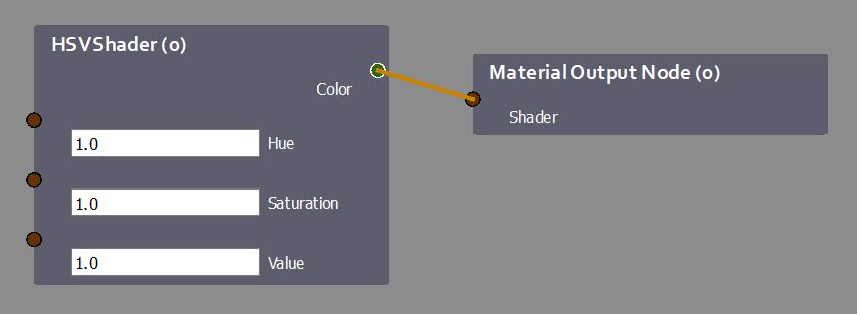
\includegraphics[width=0.7\textwidth]{img/evaluation/Simple HSV Shader Node Graph.JPG}};
\node (render) [right=of nodegraph] {
\includegraphics[width=0.2\textwidth]{img/evaluation/Simple HSV Shader Render.png}};

\draw [ultra thick, ->] (nodegraph) to (render);
\end{tikzpicture}
\caption{HSV test shader $M_1$ using a single HSV Shader node with the rendered texture to the right, using default parameters. The HSV Shader does not utilize the fragment position argument, resulting in a uniformly colored texture.}
\label{fig:M1NodeGraphAndDefaultRender}
\end{figure}

The two generated targets are presented in figures \ref{fig:TargetsHSVShaderModelTwoParam} and \ref{fig:TargetsHSVShaderModelRandom} where the former is rendered by changing only two parameters, the hue and the saturation values, and the latter is rendered by randomizing every parameter.

\begin{figure}[!h]
\centering
\begin{subfigure}{.25\textwidth}
    \centering
    
\includegraphics[width=\linewidth]{img/evaluation/hsv_target_h=0.3,s=0.6.png}
    \caption{Target texture $T_ {11}$ where the hue and saturation values are changed.}
    \label{fig:TargetsHSVShaderModelTwoParam}
\end{subfigure}\hspace{1.5cm}
\begin{subfigure}{.25\textwidth}
    \centering
    
\includegraphics[width=\linewidth]{img/evaluation/hsv_random_target h=0.06,s=0.881,v=0.501.png}
    \caption{Target texture $T_ {12}$ where all parameters have been randomized.}
    \label{fig:TargetsHSVShaderModelRandom}
\end{subfigure}
\caption{The two test target textures for HSV Test Shader model $M_1$.}
\label{fig:TargetsHSVShaderModel}
\end{figure}

\subsection{Simple Brick Shader Model $M_2$}
The next test shader $M_2$ is a basic brick shader with a total of three shader nodes: a cloud shader, HSV shader and a brick shader. The color of the bricks are controlled by a color from the HSV shader, where the \textit{value} parameter is modulated by noise from the cloud shader. The model has a total of 9 user controllable input parameters, one of which is a color vector parameter with three channels, so in reality the model depends on 11 parameters. The brick shader is fairly complex, resulting in a big leap in number of PyTorch functions used, from 17 for $M_1$ to 544 for $M_2$. The brick test shader node graph and resulting rendered texture for default parameters are displayed in Figure \ref{fig:M2NodeGraphAndDefaultRender}.

\begin{figure}[!h]
    \centering
    \begin{tikzpicture}
        \node (nodegraph) {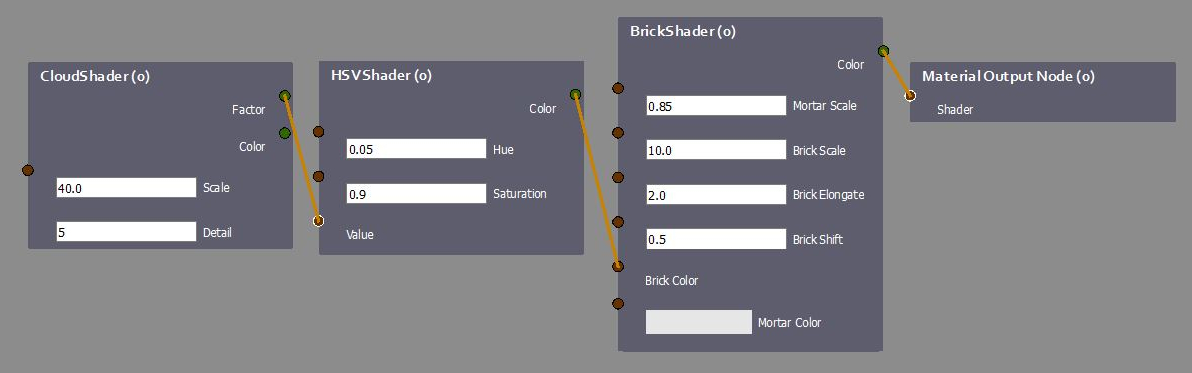
\includegraphics[width=0.7\textwidth]{img/evaluation/Brick Shader Node Graph.JPG}};
        \node (render) [right=of nodegraph] {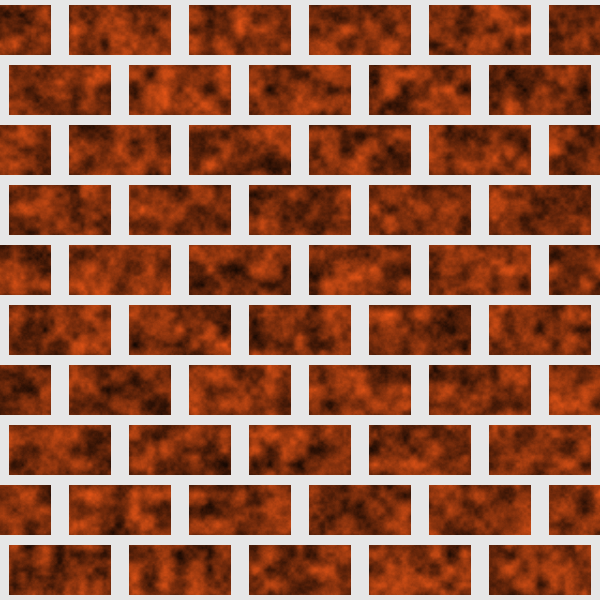
\includegraphics[width=0.2\textwidth]{img/evaluation/Brick Shader Render.png}};
        
        \draw [ultra thick, ->] (nodegraph) to (render);
    \end{tikzpicture}
    \caption{Brick shader $M_2$ using a Cloud Shader connected to a HSV Shader connected to a Brick Shader with the resulting rendered texture to the right, using default parameters. }
    \label{fig:M2NodeGraphAndDefaultRender}
\end{figure}

The two generated targets for $M_2$ are presented in figures \ref{fig:TargetM2TwoParam} and \ref{fig:TargetM2Random} respectively. The first is rendered by changing only two parameters, the elongation of the bricks and the hue of the bricks, and the last is rendered by randomizing every parameter.

\begin{figure}[!h]
\centering
\begin{subfigure}[t]{.25\textwidth}
    \centering
    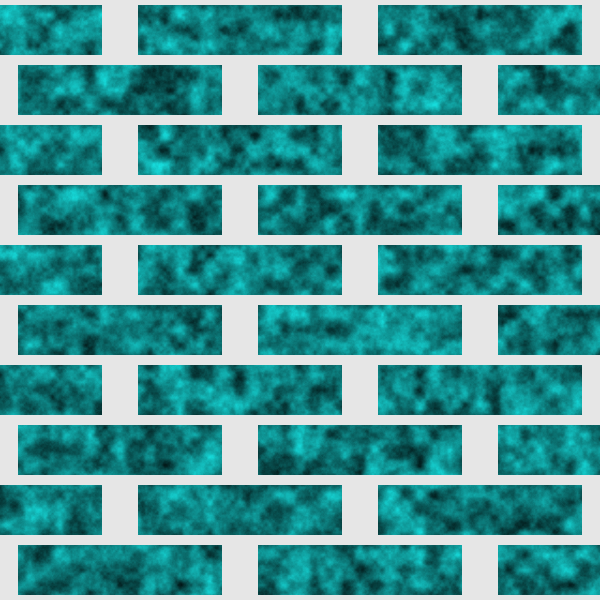
\includegraphics[width=\linewidth]{img/evaluation/simple_brick_target brick_elongate=4,hue=0.5.png}
    \caption{Target texture $T_ {21}$ where the elongation and hue of the bricks are changed.}
    \label{fig:TargetM2TwoParam}
\end{subfigure}\hspace{1.5cm}
\begin{subfigure}[t]{.25\textwidth}
    \centering
    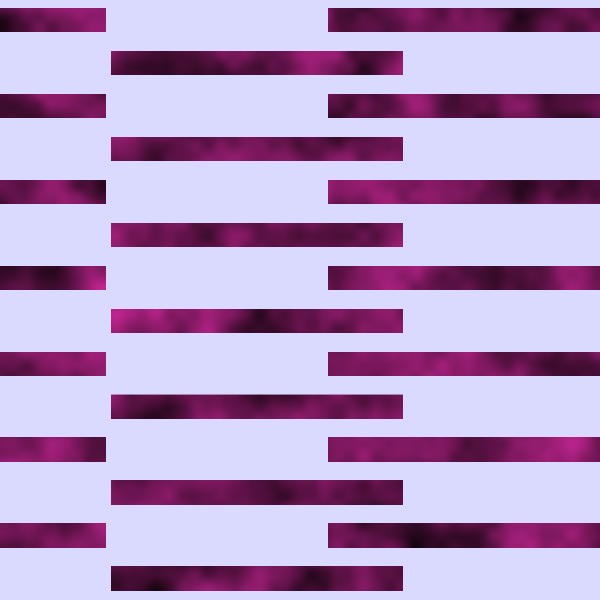
\includegraphics[width=\linewidth]{img/evaluation/simple_brick_random_target.png}
    \caption{Target texture $T_ {22}$ where every parameter is randomized.}
    \label{fig:TargetM2Random}
\end{subfigure}
\caption{The two test target textures for shader model $M_2$.}
\label{fig:TargetsM2}
\end{figure}


\subsection{Advanced Brick Shader Model $M_3$}
The final shader model $M_3$ is an advanced version of $M_2$ using a different brick shader adapted from \textit{Blender's} brick shader implementation in GLSL, as well as using classic 3D perlin noise, which is much more complex than the fractal brownian motion noise used in the cloud shaders. In total, $M_2$ depends on 26 parameters and a total of 2498 PyTorch functions. The node graph of $M_3$ and rendered texture using default parameters are shown in Figure \ref{fig:M3NodeGraphAndDefaultRender}.

\begin{figure}
    \centering
    \begin{tikzpicture}
    \node (nodegraph) {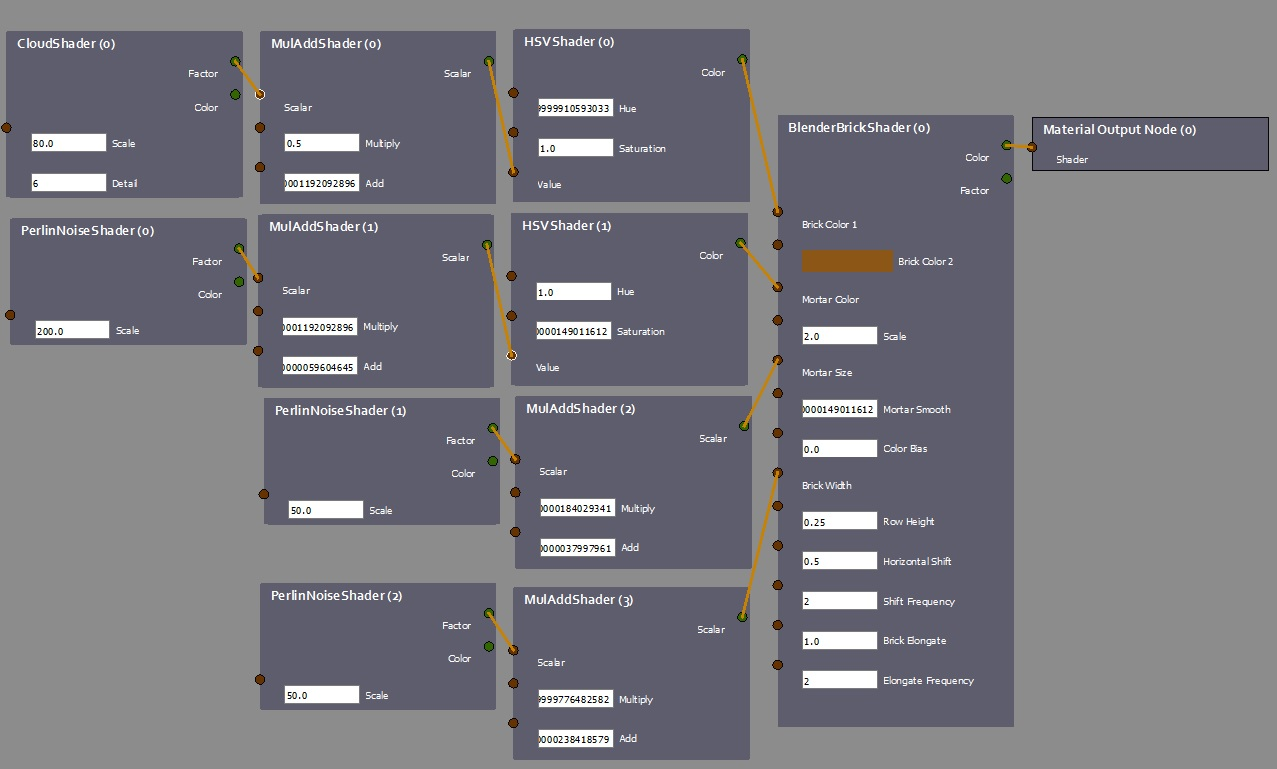
\includegraphics[width=0.7\textwidth]{img/evaluation/Advanced Brick Shader Node Graph.jpg}};
        \node (render) [right=of nodegraph] {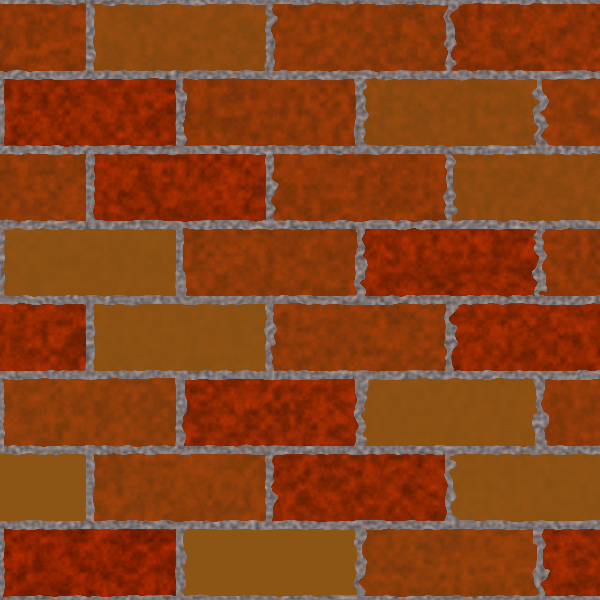
\includegraphics[width=0.2\textwidth]{img/evaluation/Advanced Brick Shader Render.png}};
        
        \draw [ultra thick, ->] (nodegraph) to (render);
    \end{tikzpicture}
    \caption{Advanced brick shader $M_3$ using an adapted version of \textit{Blender's} brick shader as well as multiple instances of classic 3D perlin noise. The resulting rendered texture using default parameters is shown on the right.}
    \label{fig:M3NodeGraphAndDefaultRender}
\end{figure}

For this shader model, we generate two targets in a fashion similar to $M_1$ and $M_2$ shown in figures \ref{fig:TargetM3T31TwoParam} and \ref{fig:TargetM3T32Random} respectively. The first image shows the target rendered by changing only two parameters, the scale of the bricks and the color bias while the second image shows a target rendered by randomizing each parameter. Additionally, this shader is advanced enough that it could render something resembling a real life texture, which is why we test it on a third, real life texture of a brick wall, shown in Figure \ref{fig:TargetM3T33RealLife}.

\begin{figure}[!h]
\centering
\begin{subfigure}[t]{.25\textwidth}
    \centering
    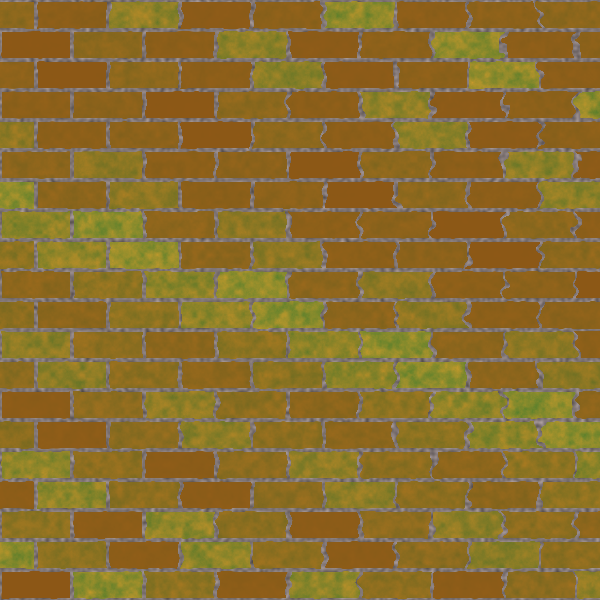
\includegraphics[width=\linewidth]{img/evaluation/adv_brick_target_scale=5,color_bias=1.png}
    \caption{Target texture $T_ {31}$ where the brick scale and color bias have been changed.}
    \label{fig:TargetM3T31TwoParam}
\end{subfigure}\hspace{0.7cm}
\begin{subfigure}[t]{.25\textwidth}
    \centering
    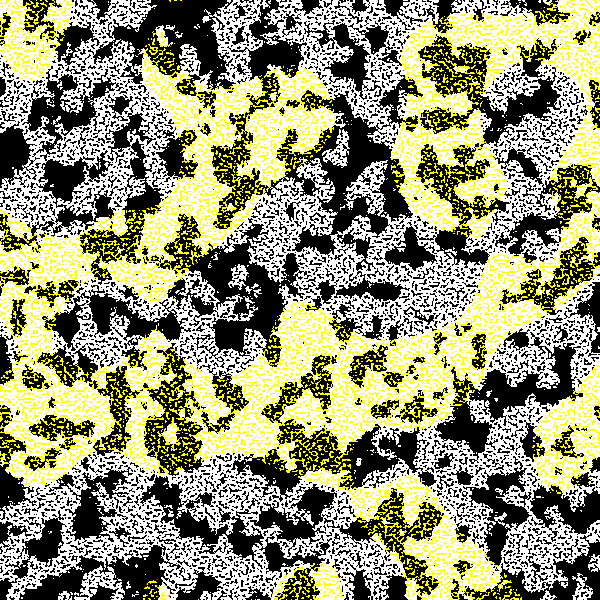
\includegraphics[width=\linewidth]{img/evaluation/adv_brick_random_target.png}
    \caption{Target texture $T_ {32}$where every parameter has been randomized.}
    \label{fig:TargetM3T32Random}
\end{subfigure}\hspace{0.7cm}
\begin{subfigure}[t]{.25\textwidth}
    \centering
    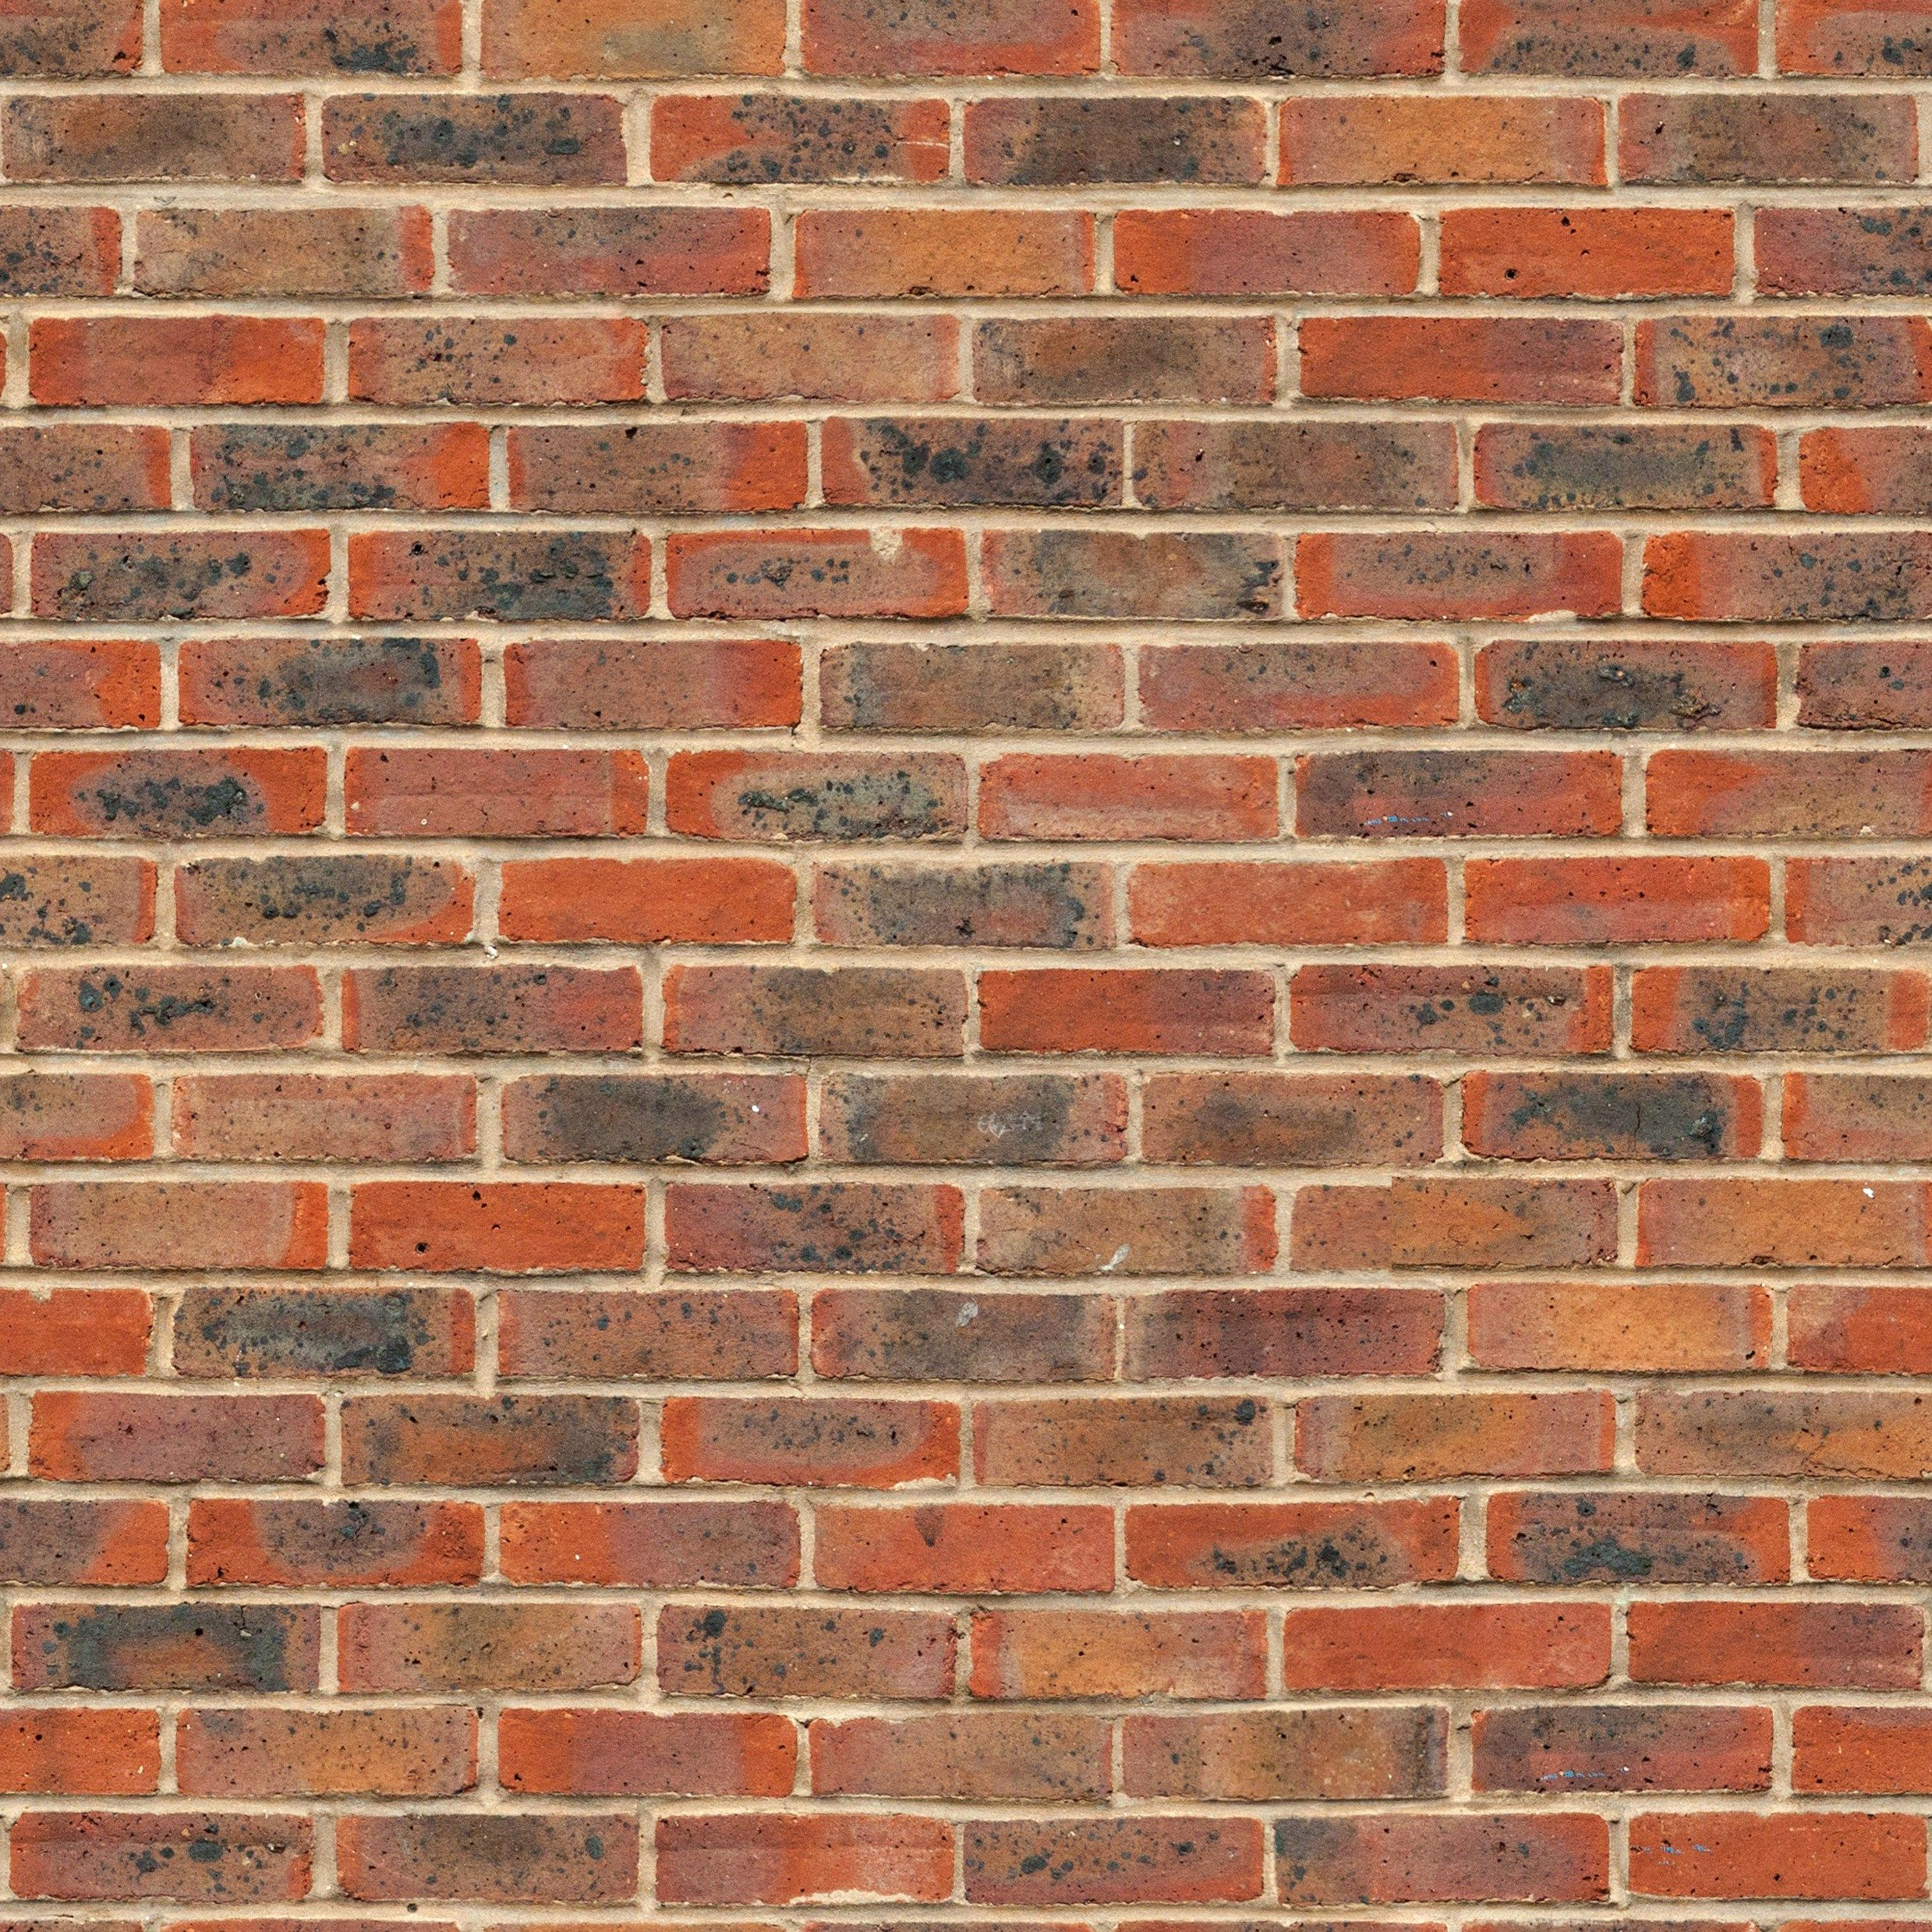
\includegraphics[width=\linewidth]{img/evaluation/adv_brick_real_life_target.jpg}
    \caption{Real life target texture (photograph) $T_{33}$ of a brick wall.}
    \label{fig:TargetM3T33RealLife}
\end{subfigure}
\caption{The three test target textures for shader model $M_3$ including an additional real life target.}
\label{fig:TargetsM3}
\end{figure}

\section{Python Rendering Performance}

The rendering time of our Python shaders can be a major bottleneck during parameter estimation as one texture image is rendered per iteration of gradient descent. The rendering performance is therefore evaluated on the three shaders models described in section \ref{sec:ShaderModelsForEvaluation} for a number of sizes. We use $150$ linearly sampled sizes between $10\times10$ and $1000\times1000$ pixels plus an additional selected size of $200\times200$ which is the default render size in \dipter{}. For each shader and render size, a texture is rendered three times and the average CPU execution time is recorded. The results are plotted in Figure \ref{fig:PythonRenderingPerformance} on a log-log plot where the y-axis shows the rendering time in milliseconds while the number of pixels is displayed on the x-axis. A dotted horizontal line shows the threshold for real time performance, here defined as rendering 30 times per second or more, equivalent to a rendering time of approximately 33ms, and a dotted vertical line marks the default rendering size of $200\times 200$ pixels.

\begin{figure}[h]
    \centering
    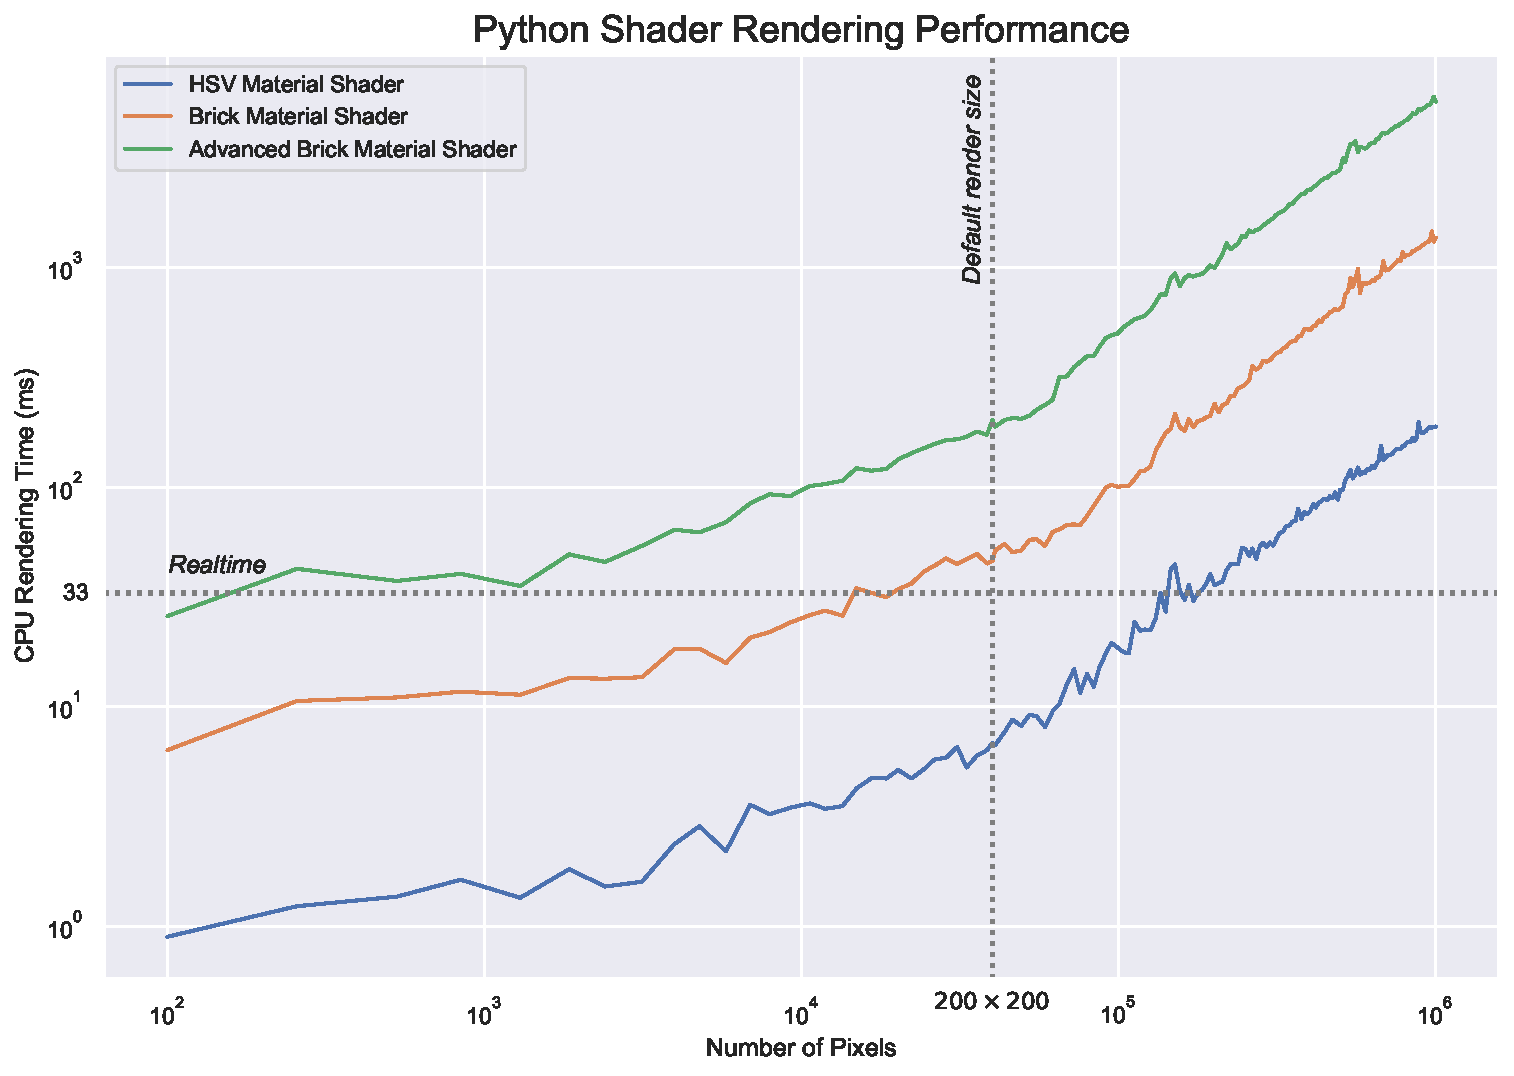
\includegraphics[width=0.9\textwidth]{img/evaluation/PythonRenderingPerformance.pdf}
    \caption{The CPU rendering time in milliseconds it takes to render an image of a certain size, measured in milliseconds per total number of pixels, for the back-end Python render engine. A horizontal dotted line indicates the threshold for real time performance ($33$ms/render) and a vertical dotted line indicates the number of pixels in the default render size ($200\times 200$ pixels).}
    \label{fig:PythonRenderingPerformance}
\end{figure}

We can observe that the rendering time scales linearly with the number of rendered pixels which is expected. Furthermore, rendering performance is largely dictated by the complexity of the shader function. For $M_1$, rendering a texture of default size, $200\times 200$, only takes around 7 milliseconds and we can achieve real time performance for up to a resolution of about $360\times 360$ pixels. For $M_2$, rendering a texture of default size takes considerably longer at about 46 milliseconds and we can only achieve real time performance for textures of up to around $116\times 116$ pixels. Lastly, for the most advanced shader function real time performance is already surpassed at a resolution of $16\times 16$ pixels and rendering a texture using the default resolution takes around 200 milliseconds. While real time performance is by no means a requirement for the Python shading, it will directly affect the time it takes to perform the parameter estimation, as seen in section \ref{sec:EvalParameterEstimation}. A constant part of the total rendering time does not directly depend on the resolution or the number of functions used, but on the number of nodes in the node graph as well as the number of inputs that have to be checked for those nodes. For $M_1$, this is about 1.5 milliseconds, for $M_2$ about 6 milliseconds and for $M_3$ about 20 milliseconds or on average about 1.8 milliseconds per node. 

\section{Parameter Estimation}\label{sec:EvalParameterEstimation}

The algorithm itself used for parameter estimation is fairly simple but needs to solve two difficult problems. First of all, we need a reliable way of finding a path towards a minimum of our loss function and unfortunately there is no way of knowing if the reached minimum is actually a global minimum or a local minimum. Second, the loss functions global minima must correspond to a satisfactory similarity between the target and generated texture, and should ideally be as smooth as possible in all dimensions. In this section, we will therefore survey different optimizer strategies, which solve the first problem, and different loss functions, pertaining to the second problem, for our three test shaders and discuss the advantages and disadvantages of the different combinations.

We rendered a texture from each of our three test shaders where only two variables have been changed, $T_{i1}$, which allows us to plot the loss as a surface dependent on these two variables and trace the parameter estimation progress along this surface. It also serves as an easy starting point of evaluation as we later evaluate parameter estimation using every variable, targets $T_{i2}$.

Evaluating the parameter estimation is done separately for each of the test shader models $M_1$, $M_2$ and $M_3$ for each possible combination of our three implemented loss functions, see section \ref{sec:MethodLossFunctions}, and optimizers. The optimizers we chose to test are the popular \textit{Adam} and the predecessor \textit{RMSprop}, both of which comes bundled with PyTorch. When performing the gradient descent, the initial state of the shader model is equivalent to that shown in the node setups in figures \ref{fig:M1NodeGraphAndDefaultRender}, \ref{fig:M2NodeGraphAndDefaultRender} and \ref{fig:M3NodeGraphAndDefaultRender} respectively. Normally when gradient descent is used to optimize a neural network the initial parameters are randomized, which is not best practice in \dipter{} as a user will typically design their shader model as far as possible and then use the parameter estimation as a final step to find even better parameter values. Randomizing initial parameters will effectively undo all of the user's progress and will in most cases result in a higher initial loss. All textures are compared as matrices where the color values are stored as floating point values ranging from $0.0$ to $1.0$. All plots follow the convention that parameter estimations for $T_{i1}$ are shown as solid lines while parameter estimations for the $T_{i2}$ targets are shown as dotted lines, additionally using blue or orange color when using Adam or RMSprop, respectively.

\subsection{Parameter Estimation Speed}\label{sec:EvalParameterEstimationSpeed}

Difficult optimization problems often require hundreds of iterations to reach a low loss value and the execution time of a loss function can thus greatly influence the overall parameter estimation time. In Figure \ref{fig:ParameterEstimationSpeed} the average iteration time per shader per loss function is presented. This data was produced by executing 10 iterations of gradient descent three times with both Adam and RMSprop and then averaging over those times. We did not separate the data between the different optimizers as there was no significant difference between them. The rendering resolution was set to $224\times224$ pixels, the required resolution of input to VGG19 used in the neural loss function, and the rendering time is included in the plot. It is clear that Mean Squared Error and Squared Bin Loss are much faster functions than the Neural Loss and the almost constant difference between their execution time suggests that the total time mainly scales with the render resolution and complexity of shader model. In cases where a neural loss function does not clearly result in a more accurate result, there is not much justification for its greater execution time. However, when the model is sufficiently complex so that the rendering time is the largest factor, in terms of iteration time, it does not matter much which loss function is used. 

\begin{figure}
    \centering
    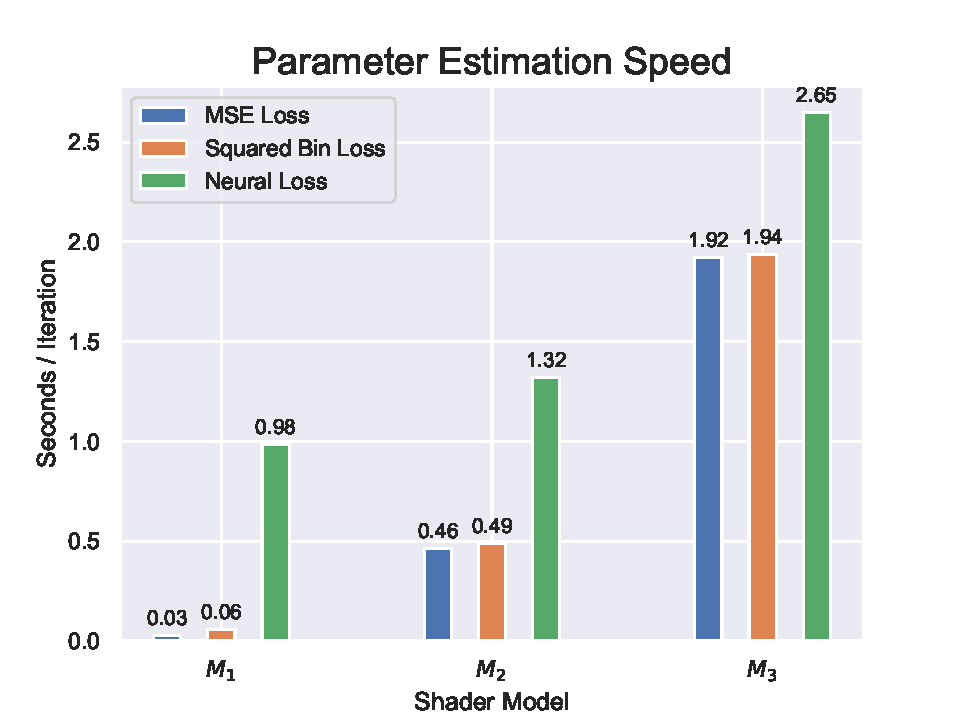
\includegraphics[width=0.9\textwidth]{img/evaluation/Parameter Estimation Speed.pdf}
    \caption{Execution time in seconds for an iteration of gradient descent for different shader models and loss functions. The iteration time includes the process of rendering an image from the shader model once using a resolution of $224\times224$ pixels.}
    \label{fig:ParameterEstimationSpeed}
\end{figure}


\subsection{Parameter Estimation using MSE}

\begin{table}[h]
\centering
\begin{tabular}{ccllllll}
\textbf{}      &                   & \textbf{}          & \multicolumn{1}{l|}{}            & \multicolumn{2}{l|}{\textit{Adam}}                           & \multicolumn{2}{l|}{\textit{RMSprop}}                      \\
\textbf{$M_i$} & \textbf{$T_{ij}$} & \textbf{Optimizer} & \multicolumn{1}{l|}{\textbf{lr}} & \textbf{$\beta_1$} & \multicolumn{1}{l|}{\textbf{$\beta_2$}} & \textbf{$\alpha$} & \multicolumn{1}{l|}{\textbf{Momentum}} \\ \hline
 $M_1$      & $T_{11}$   & Adam       & 0.15       & 0.5        & 0.999      &            &           \\
 $M_1$      & $T_{11}$   & RMSprop    & 0.09       &            &            & 0.9        & 0.0       \\
 $M_1$      & $T_{12}$   & Adam       & 0.1        & 0.5        & 0.999      &            &           \\
 $M_1$      & $T_{12}$   & RMSprop    & 0.09       &            &            & 0.9        & 0.0       \\
 $M_2$      & $T_{21}$   & Adam       & 0.05       & 0.9        & 0.999      &            &           \\
 $M_2$      & $T_{21}$   & RMSprop    & 0.01       &            &            & 0.75       & 0.4       \\
 $M_2$      & $T_{22}$   & Adam       & 0.05       & 0.8        & 0.999      &            &           \\
 $M_2$      & $T_{22}$   & RMSprop    & 0.02       &            &            & 0.75       & 0.6       \\
 $M_3$     & $T_{31}$   & Adam       & 0.05       & 0.9        & 0.999      &            &            \\
 $M_3$     & $T_{31}$   & RMSprop    & 0.01       &            &            & 0.75       & 0.4        \\
 $M_3$     & $T_{32}$   & Adam       & 0.05       & 0.8        & 0.999      &            &            \\
 $M_3$     & $T_{32}$   & RMSprop    & 0.02       &            &            & 0.75       & 0.6        \\
 $M_3$     & $T_{33}$   & Adam       & 0.04       & 0.9        & 0.999      &            &            \\
 $M_3$     & $T_{33}$   & RMSprop    & 0.01       &            &            & 0.75       & 0.4        \\
\end{tabular}
\caption{Optimizer and loss function settings when running gradient descent using Mean Squared Error loss.}
\label{tab:MSEOptimizerSettings}
\end{table}

Mean Squared Error is a loss function that measures the difference in color values for each channel and pixel between our generated image $\hat{X}$ and target $X$. \hl{It is a very simple loss function and is such much faster than, for example, a neural loss function and is well suited for} finding the similarity between simple textures without patterns as it heavily depends on spatial information. The minimum loss value that can be achieved is $0.0$ corresponding to an exact match in color values and the maximum loss is $1.0$ corresponding to a maximum difference between each pixel which stems from our use of a floating point image format. The settings used for each shader model and optimizer when evaluating Mean Squared Error loss is presented in table \ref{tab:MSEOptimizerSettings}. Each optimizer and target requires different settings to perform well and typically, a more difficult problem requires a lower learning rate and more iterations to optimize successfully.

\subsubsection{HSV Test Shader $M_1$}

\begin{figure}[ht]
    \centering
    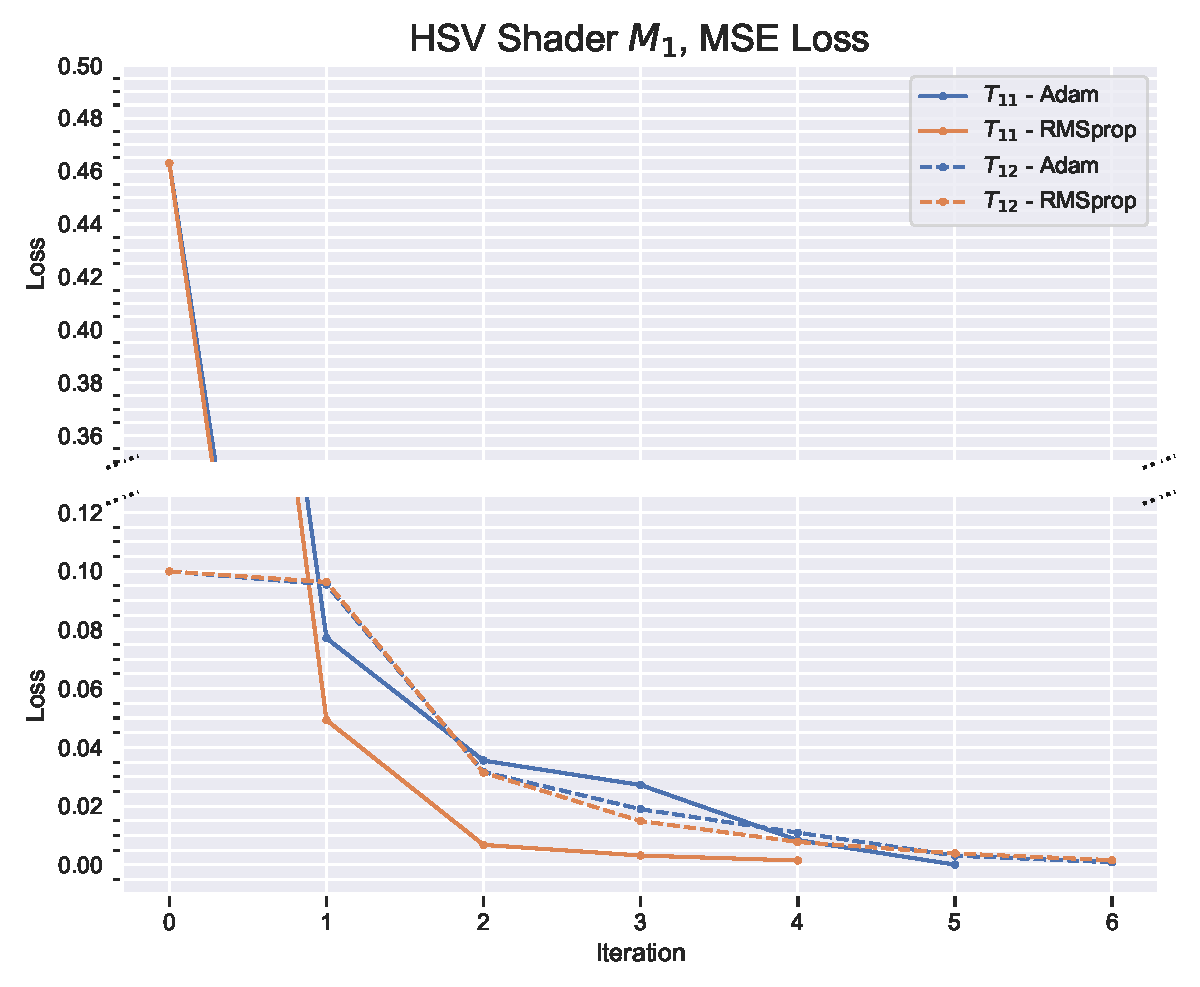
\includegraphics[width=0.8\textwidth]{img/evaluation/M1/HSV_MSE.pdf}
    \caption{Results of evaluating parameter estimation of material $M_1$ using Mean Squared Error loss. The runs with target $T_{11}$ are plotted as solid lines while runs with target $T_{12}$ are plotted with dashed lines.}
    \label{fig:M1MSEData}
\end{figure}

First, parameter estimation using an MSE loss function with $M_1$ is evaluated and the results are shown in Figure \ref{fig:M1MSEData}. The target loss threshold is set to $0.0025$ corresponding to an average difference in color values of $\sqrt{0.0025}=0.05$ or $5\%$. We are able to reach the loss threshold in only a few iterations using either optimization methods. As expected, a few more iterations are required to reach the threshold for target $T_{12}$ as more parameters have to be optimized, even though the initial loss is actually lower than for $T_{11}$. Furthermore, a simple model like $M_1$ seems to be more efficiently optimized using RMSprop than the more modern Adam, possibly due to Adam requiring a few initial iterations in order to build up momentum. For this experiment, using a learning rate of under $1.0$ proved a necessity for RMSprop, where using a larger value resulted in a divergence of the loss. Lowering the first moment parameter $\beta_1$ for Adam proved very helpful in order to diminish its oscillating behaviour. Typically, MSE is not a very good loss function for image comparison, but as $M_1$ is uniform across the entire image, the spatial dependence of MSE is not a problem and proves very efficient for similar problems.

\subsubsection{Simple Brick Test Shader $M_2$}
\begin{figure}[hp]
    \centering
    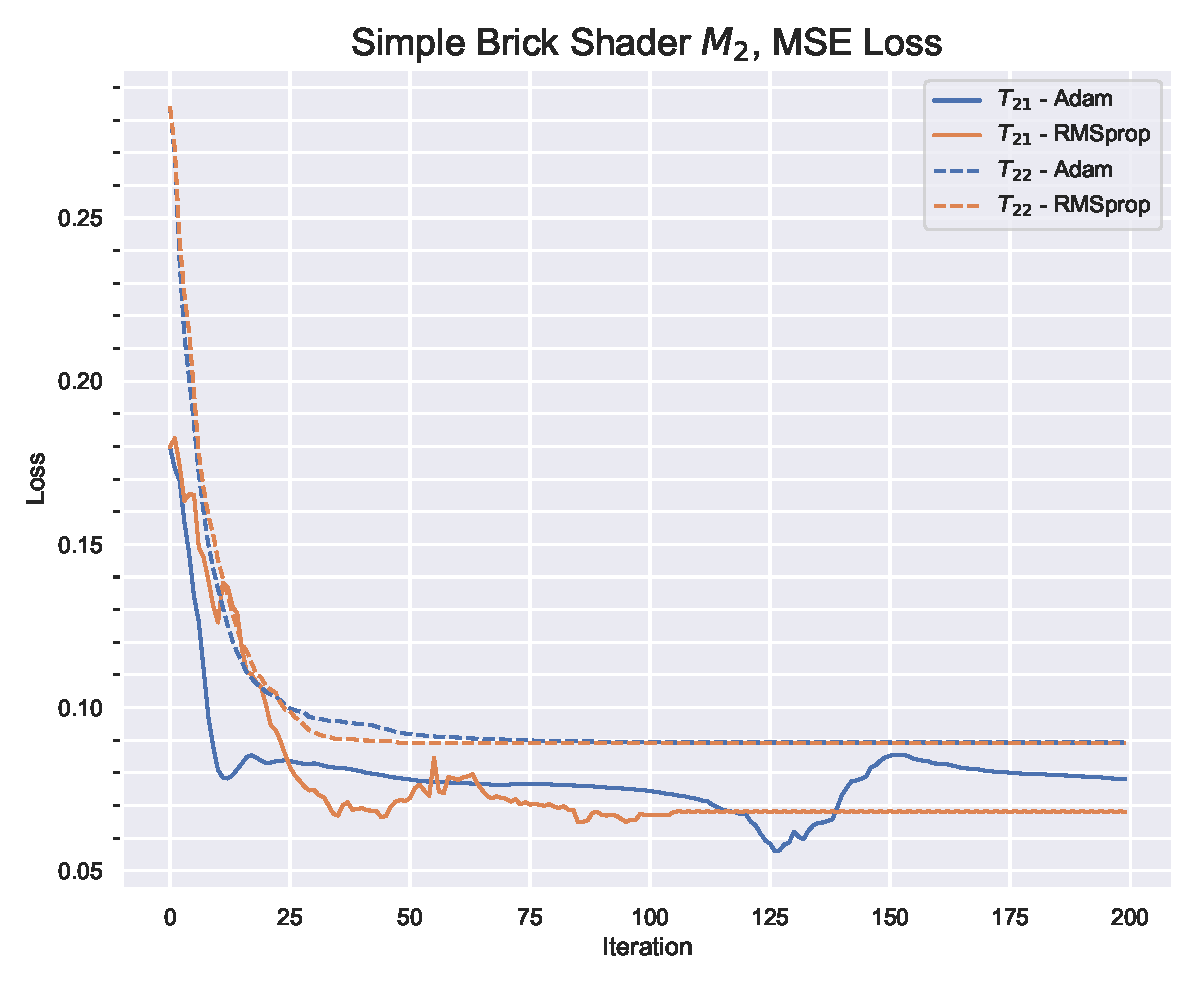
\includegraphics[width=0.8\textwidth]{img/evaluation/M2/SBS_MSE.pdf}
    \caption{Results of evaluating parameter estimation of material $M_2$ using Mean Squared Error loss. The runs with target $T_{21}$ are plotted as solid lines while runs with target $T_{22}$ are plotted with dashed lines.}
    \label{fig:M2MSEData}
\end{figure}

\begin{figure}[hp]
\centering
\begin{subfigure}[t]{.25\textwidth}
    \centering
    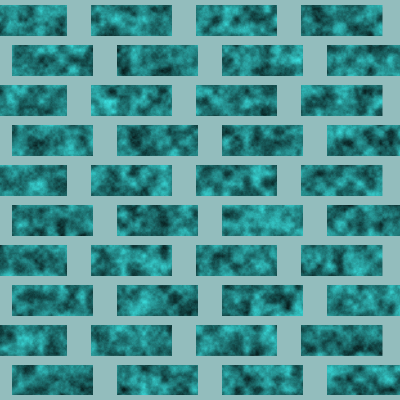
\includegraphics[width=\linewidth]{img/evaluation/M2/2param/MSE_Adam_final_render.png}
    \caption{Target $T_{21}$ using Adam.}
    \label{fig:M2MSEFinalRenders2paramAdam}
\end{subfigure}\hspace{0.7cm}
\begin{subfigure}[t]{.25\textwidth}
    \centering
    
\includegraphics[width=\linewidth]{img/evaluation/M2/random/MSE_Adam_random_final_render.png}
    \caption{Target $T_{22}$ using Adam.}
    \label{fig:M2MSEFinalRendersRandomAdam}
\end{subfigure}
\vskip\baselineskip
\begin{subfigure}[t]{.25\textwidth}
    \centering
    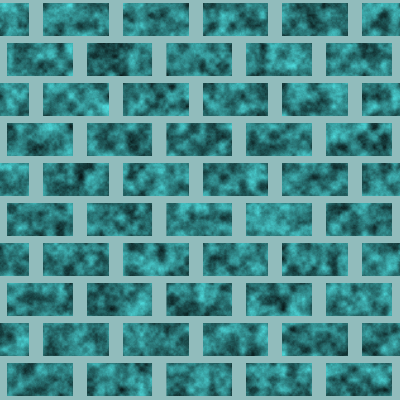
\includegraphics[width=\linewidth]{img/evaluation/M2/2param/MSE_RMSprop_final_render.png}
    \caption{Target $T_{21}$ using RMSprop.}
    \label{fig:M2MSEFinalRenders2paramRMSprop}
\end{subfigure}\hspace{0.7cm}
\begin{subfigure}[t]{.25\textwidth}
    \centering
    
\includegraphics[width=\linewidth]{img/evaluation/M2/random/MSE_RMSprop_random_final_render.png}
    \caption{Target $T_{22}$ using RMSprop.}
    \label{fig:M2MSEFinalRendersRandomRMSprop}
\end{subfigure}
\caption{The four rendered textures at the point of minimal loss for $M_2$ using MSE loss corresponding to the four plots in Figure \ref{fig:M2MSEData} with combinations of optimizers Adam or RMSprop and targets $T_{21}$ or $T_{22}$.}
\label{fig:M2MSEFinalRenders}
\end{figure}

Next, we use the MSE loss function to estimate parameters for the more complex brick shader model $M_2$. Unlike $M_1$ this model is not uniform accross the image and features lots of patterns and even pseudorandom noise which MSE is very ill equipped to handle. Looking at the resulting data in Figure \ref{fig:M2MSEData} we can see that for target $T_{21}$ we are able to find a parameter set that significantly lowers the loss value from around $0.18$ down to a minimum of $0.056$ at iteration 126 for Adam and $0.065$ for RMSprop significantly earlier at iteration 85. In all four cases we lowered the learning rate compared to $M_1$ as this is a more difficult problem with more parameters, as well as increased the $\beta_1$ value to $0.9$ in order to stabilize the progress. Momentum was also utilized here for RMSprop which seemed to help with finding a slightly better minimum. As stated before, MSE is not a good choice for images with patterns but can be efficient at finding the overall color tone of the image. For both optimizers for target $T_{21}$ the blue color of the bricks are successfully reproduced, but not the brick shape, even though Adam managed to produce a result with slightly elongated bricks. As expected, the optimization for target $T_{22}$ was not as successful and did only reach a minimum loss of about $0.089$ for both optimizers which converged around iteration 75. The final renders with the optimized parameters are shown in Figure \ref{fig:M2MSEFinalRenders}. For a relatively complex shader like $M_2$ it seems to be only possible to reproduce the overall color tone of the target texture, but any pattern is either completely lost as in renders \ref{fig:M2MSEFinalRendersRandomAdam} and \ref{fig:M2MSEFinalRendersRandomRMSprop} or the shape is not correctly recovered as in renders \ref{fig:M2MSEFinalRenders2paramAdam} and \ref{fig:M2MSEFinalRenders2paramRMSprop}.

\subsubsection{Advanced Brick Test Shader $M_3$}
\begin{figure}[hp]
    \centering
    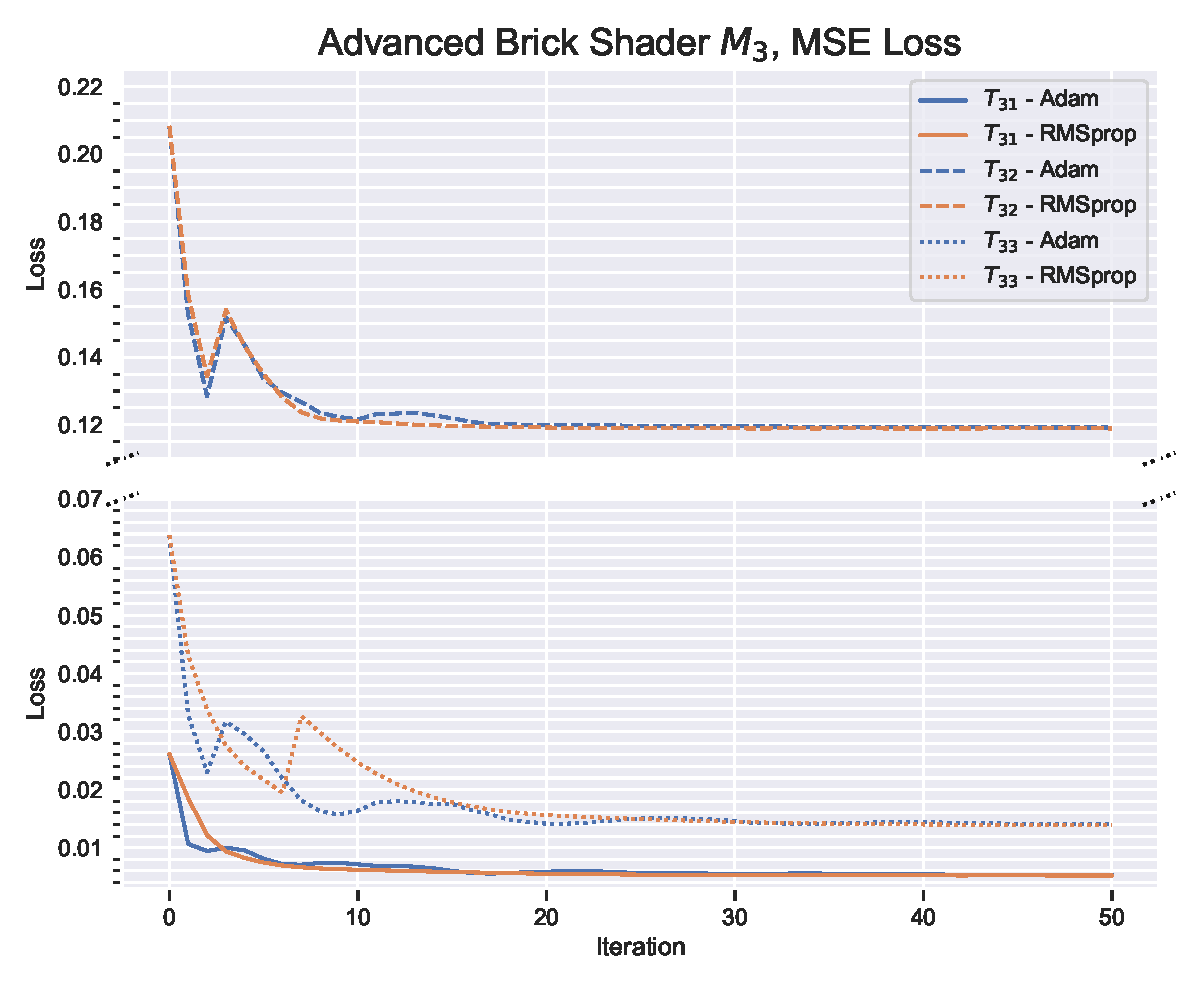
\includegraphics[width=0.8\textwidth]{img/evaluation/M3/ABS_MSE.pdf}
    \caption{Results of evaluating parameter estimation of material $M_3$ using Mean Squared Error loss. The runs with target $T_{31}$ are plotted as solid lines, target $T_{32}$ with dashed lines and the additional real-life target $T_{33}$ with dotted lines. The iterations have been truncated from 200 to 50 iterations as the loss converges before iteration 50.}
    \label{fig:M3MSEData}
\end{figure}

Finally test shader $M_3$ is evaluated using the MSE loss function and the results are shown in Figure \ref{fig:M3MSEData} and best renders in Figure \ref{fig:M3MSEFinalRenders} where the same optimizer settings were used as with $M_2$ for targets $T_{31}$ and $T_{32}$. For target $T_{31}$, the initial loss is relatively low at just above $0.025$ and both optimizers reaches a minimum loss of $0.0052$, fairly close to our threshold of $0.0025$. This demonstrates the fact that MSE often does not correspond with how humans judge similarity, because when comparing the initial render in \ref{fig:M3NodeGraphAndDefaultRender} and the target $T_{31}$ in \ref{fig:TargetM3T31TwoParam} they clearly portray very different brick walls. The optimization looks rather successful on paper, but looking at the render from the parameters at the point of minimal loss in Figure \ref{fig:M3MSEFinalRenders}, only the average color has been captured. As expected, the performance for target $T_{32}$ using random parameters is worse, only reaching a minimum loss of about $0.12$ around iteration 20 for either optimizer. The additional real-life target $T_{33}$ plotted with dotted lines lies somewhere in between, starting with a loss of about $0.065$ and converging to a loss of about $0.014$. The same behaviour is shown here as seen before, where the renders in sub-figures \ref{fig:M3MSEFinalRendersRealLifeAdam} and \ref{fig:M3MSEFinalRendersRealLifeRMSprop} show that the MSE loss only restores the overall color of the target. Clearly a Mean Squared Error loss is not optimal when estimating parameters for complex shaders with an extensive use of patterns.  
\begin{figure}[h]
\centering
\begin{subfigure}[t]{.25\textwidth}
    \centering
    
\includegraphics[width=\linewidth]{img/evaluation/M3/2 param/MSE_Adam_2_param_final.png}
    \caption{Target $T_{31}$ using Adam.}
    \label{fig:M3MSEFinalRendersTwoParamAdam}
\end{subfigure}\hspace{0.7cm}
\begin{subfigure}[t]{.25\textwidth}
    \centering
    
\includegraphics[width=\linewidth]{img/evaluation/M3/random/MSE_Adam_random_final.png}
    \caption{Target $T_{32}$ using Adam.}
    \label{fig:M3MSEFinalRendersRandomAdam}
\end{subfigure}\hspace{0.7cm}
\begin{subfigure}[t]{.25\textwidth}
    \centering
    
\includegraphics[width=\linewidth]{img/evaluation/M3/real life/MSE_Adam_real_life_final.png}
    \caption{Target $T_{33}$ using Adam.}
    \label{fig:M3MSEFinalRendersRealLifeAdam}
\end{subfigure}
\vskip\baselineskip
\begin{subfigure}[t]{.25\textwidth}
    \centering
    
\includegraphics[width=\linewidth]{img/evaluation/M3/2 param/MSE_RMSprop_2_param_final.png}
    \caption{Target $T_{31}$ using RMSprop.}
    \label{fig:M3MSEFinalRendersTwoParamRMSprop}
\end{subfigure}\hspace{0.7cm}
\begin{subfigure}[t]{.25\textwidth}
    \centering
    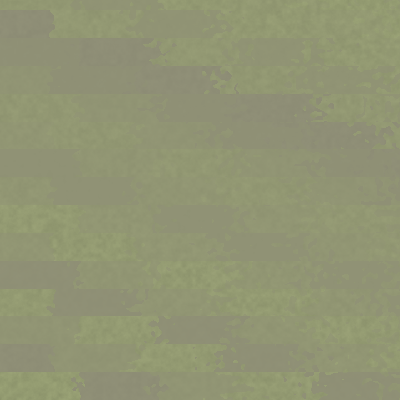
\includegraphics[width=\linewidth]{img/evaluation/M3/random/MSE_RMSprop_random_final.png}
    \caption{Target $T_{32}$ using RMSprop.}
    \label{fig:M3MSEFinalRendersRandomRMSprop}
\end{subfigure}\hspace{0.7cm}
\begin{subfigure}[t]{.25\textwidth}
    \centering
    
\includegraphics[width=\linewidth]{img/evaluation/M3/real life/MSE_RMSprop_real_life_final.png}
    \caption{Target $T_{33}$ using RMSprop.}
    \label{fig:M3MSEFinalRendersRealLifeRMSprop}
\end{subfigure}
\caption{The six rendered textures at the point of minimal loss for $M_3$ using an MSE loss function corresponding to the six plots in Figure \ref{fig:M3MSEData} with combinations of optimizers Adam or RMSprop and targets $T_{31}$, $T_{32}$ or $T_{33}$.}
\label{fig:M3MSEFinalRenders}
\end{figure}

\subsection{Parameter Estimation using Squared Bin Loss}

\begin{table}[h]
\centering
\begin{tabular}{cclllllll}
\textbf{}      &                   & \textbf{}          & \multicolumn{1}{l|}{}            & \multicolumn{2}{l|}{\textit{Adam}}                           & \multicolumn{2}{l|}{\textit{RMSprop}}                      & \multicolumn{1}{l|}{\textit{SBL}}      \\
\textbf{$M_i$} & \textbf{$T_{ij}$} & \textbf{Optimizer} & \multicolumn{1}{l|}{\textbf{lr}} & \textbf{$\beta_1$} & \multicolumn{1}{l|}{\textbf{$\beta_2$}} & \textbf{$\alpha$} & \multicolumn{1}{l|}{\textbf{Momentum}} & \multicolumn{1}{l|}{\textbf{Bin Size}} \\ \hline
 $M_1$      & $T_{11}$   & Adam       & 0.15       & 0.5        & 0.999      &            &            & 10        \\
 $M_1$      & $T_{11}$   & RMSprop    & 0.09       &            &            & 0.9        & 0.0        & 10        \\
 $M_1$      & $T_{12}$   & Adam       & 0.1        & 0.5        & 0.999      &            &            & 10        \\
 $M_1$      & $T_{12}$   & RMSprop    & 0.09       &            &            & 0.9        & 0.0        & 10        \\
 $M_2$     & $T_{21}$   & Adam       & 0.03       & 0.8        & 0.999      &            &            & 8          \\
 $M_2$     & $T_{21}$   & RMSprop    & 0.02       &            &            & 0.9        & 0.4        & 8          \\
 $M_2$     & $T_{22}$   & Adam       & 0.03       & 0.8        & 0.999      &            &            & 8          \\
 $M_2$     & $T_{22}$   & RMSprop    & 0.02       &            &            & 0.9        & 0.4        & 8          \\
  $M_3$     & $T_{31}$   & Adam       & 0.03       & 0.8        & 0.999      &            &            & 8          \\
 $M_3$     & $T_{31}$   & RMSprop    & 0.015      &            &            & 0.99       & 0.4        & 8          \\
 $M_3$     & $T_{32}$   & Adam       & 0.03       & 0.8        & 0.999      &            &            & 8          \\
 $M_3$     & $T_{32}$   & RMSprop    & 0.01       &            &            & 0.99       & 0.2        & 8          \\
\end{tabular}
\caption{Optimizer and loss settings when running gradient descent using Squared Bin loss.}
\label{tab:SBLOptimizerSettings}
\end{table}

Squared Bin Loss or SBL is effectively a version of Mean Squared Error that first downscales images into squared bins of a user controllable size and calculates the mean of each bin before returning the Mean Squared Error of the averages. This allows the loss function to better judge image similarity without comparing every pixel individually and can for some types of images help discern underlying patterns among noise. The loss value limits are the same as for the MSE loss, a minimum loss of $0.0$ and a maximum loss of $1.0$. Unlike MSE however, a loss value of $0.0$ for SBL does not necessarily mean that the images are identical, simply that the average of each bin is identical. The optimizer settings used when running gradient descent for SBL is presented in table \ref{tab:SBLOptimizerSettings}.

\newpage
\subsubsection{HSV Test Shader $M_1$}

\begin{figure}[hpt]
    \centering
    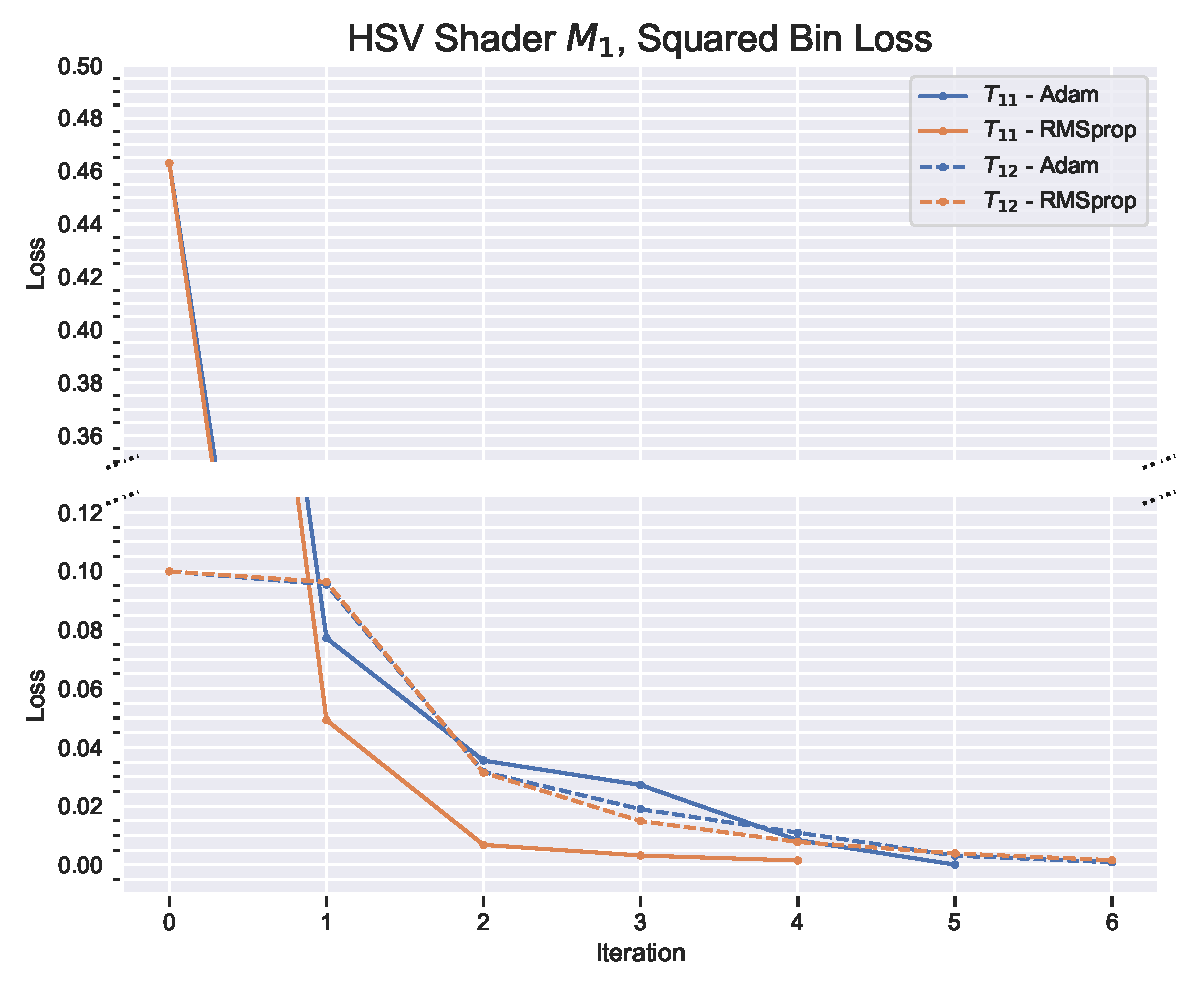
\includegraphics[width=0.8\textwidth]{img/evaluation/M1/HSV_SBL.pdf}
    \caption{Results of evaluating parameter estimation of material $M_1$ using Squared Bin loss. The runs with target $T_{11}$ are plotted as solid lines while runs with target $T_{12}$ are plotted with dashed lines.}
    \label{fig:M1SBLData}
\end{figure}

For uniform textures like those produced by $M_1$, SBL should give exactly the same result as a normal MSE loss, which is why it is curious that the loss threshold is reached, on average, one iteration earlier for SBL than MSE as shown in Figure \ref{fig:M1SBLData}, even if the exact same optimizer settings are used. This is probably more or less the result of chance, as the gradients are affected by the additional PyTorch functions used and so even if the same loss value is returned for the same data, the gradients are slightly different. Generally, this loss works equally well for uniform shaders as MSE and we were able to reach the loss threshold of $0.0025$ for both targets in five or less iterations. Similar to using MSE loss, RMSprop managed to slightly outperform Adam in this simple use case as well.

\subsubsection{Simple Brick Test Shader $M_2$}

\begin{figure}[hpb]
    \centering
    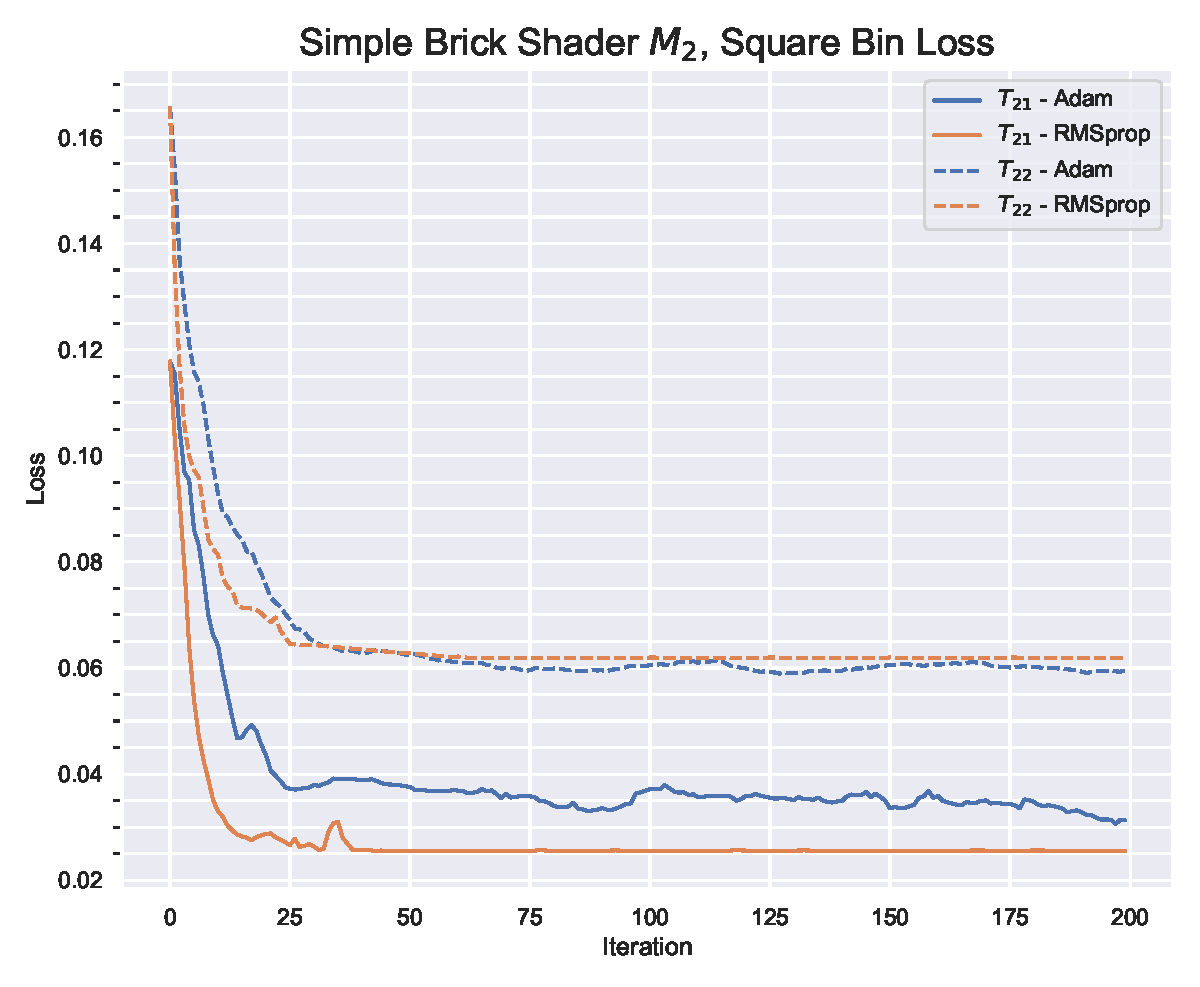
\includegraphics[width=0.8\textwidth]{img/evaluation/M2/SBS_SBL.pdf}
    \caption{Results of evaluating parameter estimation of material $M_2$ using Squared Bin loss. The runs with target $T_{21}$ are plotted as solid lines while runs with target $T_{22}$ are plotted with dashed lines.}
    \label{fig:M2SBLData}
\end{figure}

\begin{figure}[h]
\centering
\begin{subfigure}[t]{.25\textwidth}
    \centering
    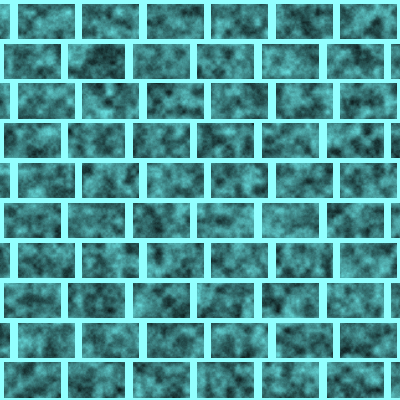
\includegraphics[width=\linewidth]{img/evaluation/M2/2param/SBL_Adam_two_param_final.png}
    \caption{Target $T_{21}$ using Adam.}
    \label{fig:M2SBLFinalRenders2paramAdam}
\end{subfigure}\hspace{0.5cm}
\begin{subfigure}[t]{.25\textwidth}
    \centering
    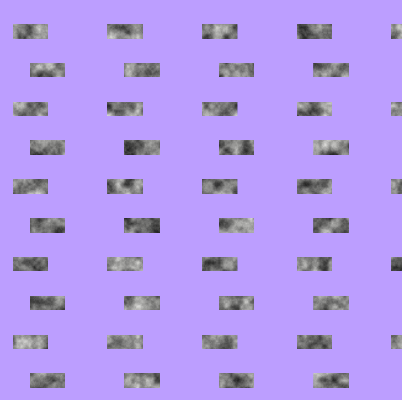
\includegraphics[width=\linewidth]{img/evaluation/M2/random/SBL_Adam_random_final.png}
    \caption{Target $T_{22}$ using Adam.}
    \label{fig:M2SBLFinalRendersRandomAdam}
\end{subfigure}
\vskip\baselineskip
\begin{subfigure}[t]{.25\textwidth}
    \centering
    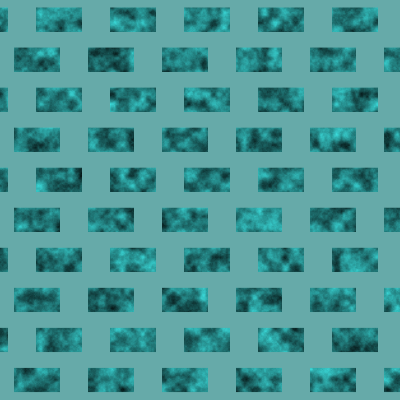
\includegraphics[width=\linewidth]{img/evaluation/M2/2param/SBL_RMSprop_two_param_final.png}
    \caption{Target $T_{21}$ using RMSprop.}
    \label{fig:M2SBLFinalRenders2paramRMSprop}
\end{subfigure}
\hspace{0.5cm}
\begin{subfigure}[t]{.25\textwidth}
    \centering
    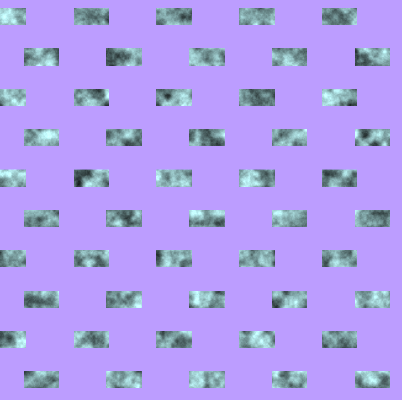
\includegraphics[width=\linewidth]{img/evaluation/M2/random/SBL_RMSprop_random_final.png}
    \caption{Target $T_{22}$ using RMSprop.}
    \label{fig:M2SBLFinalRendersRandomRMSprop}
\end{subfigure}
\caption{The four rendered textures at the point of minimal loss for $M_2$ using SBL corresponding to the six plots in Figure \ref{fig:M2SBLData} with combinations of optimizers Adam or RMSprop and targets $T_{21}$ or $T_{32}$.}
\label{fig:M2SBLFinalRenders}
\end{figure}

For test shader $M_2$ we used much lower learning rates than for $M_1$ and a higher $\beta_1$ for Adam while adding some momentum for RMSprop. The bin size was set to $8$ meaning bins of $8\times 8$ pixels are averaged, as lower values did not contribute to the accuracy and larger values would introduce too much averaging and thereby lose detail. The results are shown in Figure \ref{fig:M2SBLData} where it is apparent that for target $T_{21}$ RMSprop is outperforming Adam by a significant amount. At iteration 45 RMSprop has reached its best loss value of approximately $0.025$ while Adam reaches its best loss value of $0.03$ at iteration 197. For target $T_{22}$ the results are more even, Adam reaching a loss of around $0.059$ at iteration 127 while RMSprop reaches a loss of around $0.062$ at iteration 146. In Figure \ref{fig:M2SBLFinalRenders} we can see that the results are similar to those for MSE; the overall color has been captured, at the expense of the background color, but not the shape of the bricks although the results look slightly better for target $T_{22}$ where the bricks have been conserved but scaled down.

\subsubsection{Advanced Brick Test Shader $M_3$}

\begin{figure}[hp]
    \centering
    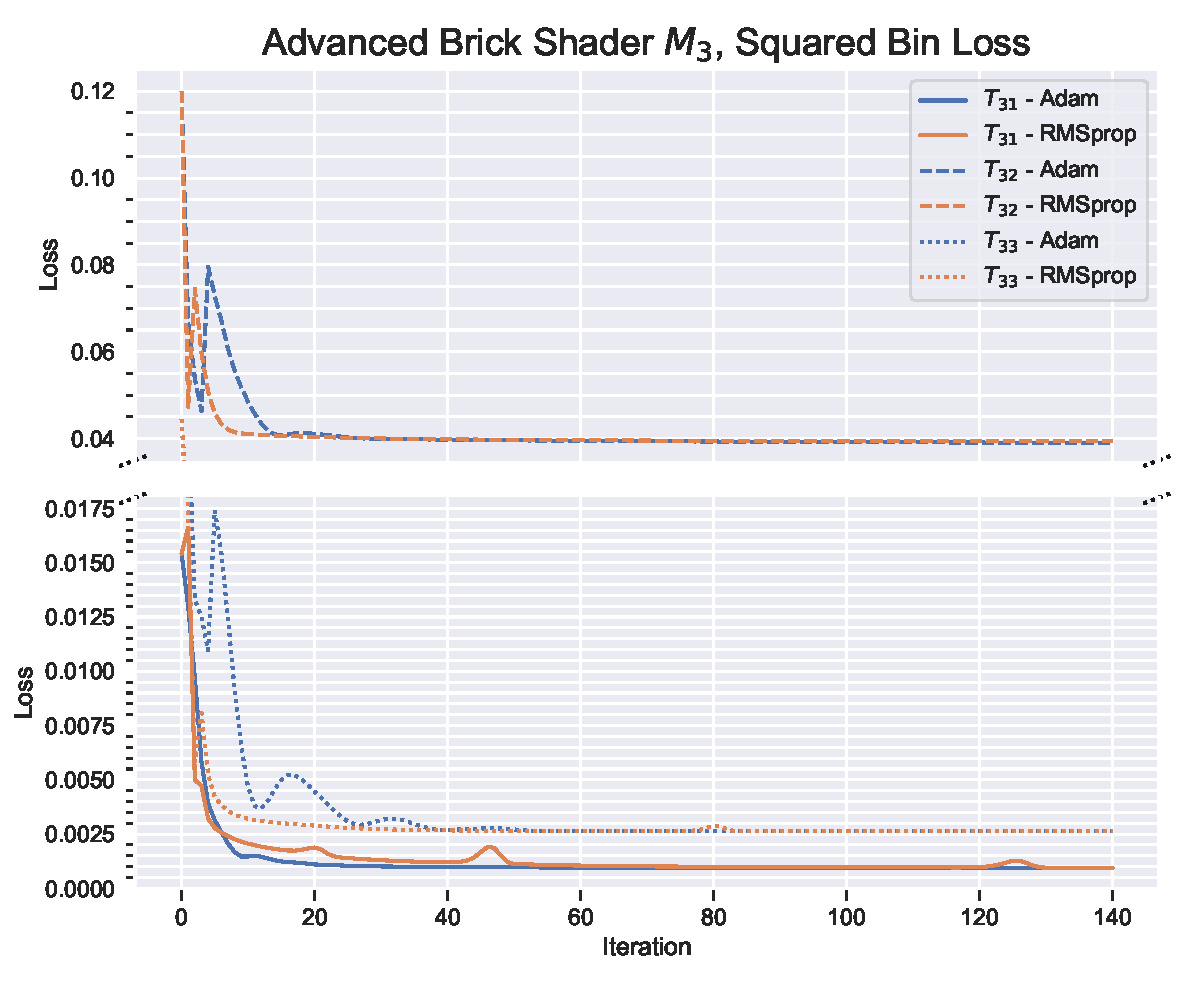
\includegraphics[width=0.8\textwidth]{img/evaluation/M3/ABS_SBL.pdf}
    \caption{Results of evaluating parameter estimation of material $M_3$ using Squared Bin loss. The runs with target $T_{31}$ are plotted as solid lines, target $T_{32}$ with dashed lines and the additional real-life target $T_{33}$ with dotted lines.}
    \label{fig:M3SBLData}
\end{figure}

For parameter estimation using SBL on shader $M_3$, similar settings to $M_2$ were used and the bin size was kept at 8. The results are shown in Figure \ref{fig:M3SBLData} and the best loss renders in Figure \ref{fig:M3SBLFinalRenders}. For both the two-parameter target $T_{31}$ and the real life target $T_{33}$ the final loss is relatively low at $0.001$ and $0.0026$ respectively for both optimizers. However, this is fairly easily achievable due to the targets having an obvious and uniform color scheme, which was restored at the expense of the bricks themselves disappearing, as the optimizer could reach a low loss value simply by assigning each pixel the average color for that bin. The results for the random target $T_{32}$ are not very satisfactory and poses a very difficult minimization problem due to the amount of noise in the image. 

\begin{figure}[hpt]
\centering
\begin{subfigure}[t]{.25\textwidth}
    \centering
    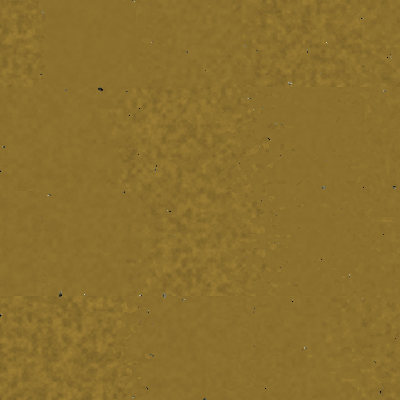
\includegraphics[width=\linewidth]{img/evaluation/M3/2 param/SBL_Adam_2param_final.png}
    \caption{Target $T_{31}$ using Adam.}
    \label{fig:M3SBLFinalRendersTwoParamAdam}
\end{subfigure}\hspace{0.7cm}
\begin{subfigure}[t]{.25\textwidth}
    \centering
    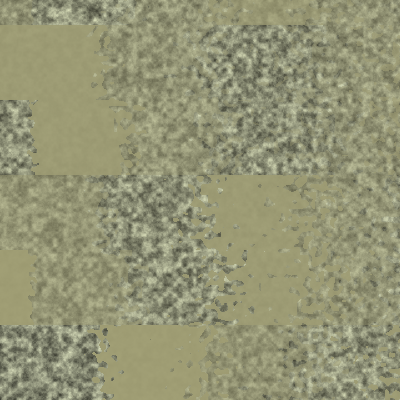
\includegraphics[width=\linewidth]{img/evaluation/M3/random/SBL_Adam_random_final.png}
    \caption{Target $T_{32}$ using Adam.}
    \label{fig:M3SBLFinalRendersRandomAdam}
\end{subfigure}\hspace{0.7cm}
\begin{subfigure}[t]{.25\textwidth}
    \centering
    
\includegraphics[width=\linewidth]{img/evaluation/M3/real life/SBL_Adam_real_life_final.png}
    \caption{Target $T_{33}$ using Adam.}
    \label{fig:M3SBLFinalRendersRealLifeAdam}
\end{subfigure}
\vskip\baselineskip
\begin{subfigure}[t]{.25\textwidth}
    \centering
    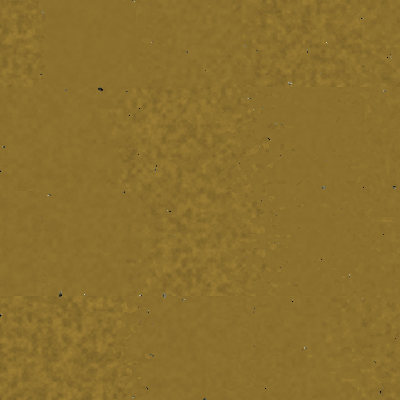
\includegraphics[width=\linewidth]{img/evaluation/M3/2 param/SBL_Adam_2param_final.png}
    \caption{Target $T_{31}$ using RMSprop.}
    \label{fig:M3SBLFinalRendersTwoParamRMSprop}
\end{subfigure}\hspace{0.7cm}
\begin{subfigure}[t]{.25\textwidth}
    \centering
    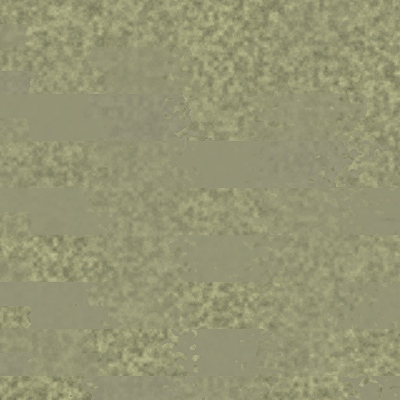
\includegraphics[width=\linewidth]{img/evaluation/M3/random/SBL_RMSprop_random_final.png}
    \caption{Target $T_{32}$ using RMSprop.}
    \label{fig:M3SBLFinalRendersRandomRMSprop}
\end{subfigure}\hspace{0.7cm}
\begin{subfigure}[t]{.25\textwidth}
    \centering

\includegraphics[width=\linewidth]{img/evaluation/M3/real life/SBL_RMSprop_real_life_final.png}
    \caption{Target $T_{33}$ using RMSprop.}
    \label{fig:M3SBLFinalRendersRealLifeRMSprop}
\end{subfigure}
\caption{The six rendered textures at the point of minimal loss for $M_3$ using SBL corresponding to the six plots in Figure \ref{fig:M3SBLData} with combinations of optimizers Adam or RMSprop and targets $T_{31}$, $T_{32}$ or $T_{33}$.}
\label{fig:M3SBLFinalRenders}
\end{figure}

\newpage
\subsection{Parameter Estimation using Neural Loss}

\begin{table}[!h]
\centering
\begin{tabular}{ccllllllll}
\textbf{}      &                   & \textbf{}          & \multicolumn{1}{l|}{}            & \multicolumn{2}{l|}{\textit{Adam}}                           & \multicolumn{2}{l|}{\textit{RMSprop}}                      & \multicolumn{2}{l|}{\textit{Neural Loss}}               \\
\textbf{$M_i$} & \textbf{$T_{ij}$} & \textbf{Optimizer} & \multicolumn{1}{l|}{\textbf{lr}} & \textbf{$\beta_1$} & \multicolumn{1}{l|}{\textbf{$\beta_2$}} & \textbf{$\alpha$} & \multicolumn{1}{l|}{\textbf{Momentum}} & \textbf{layers} & \multicolumn{1}{l|}{\textbf{weights}} \\ \hline
 $M_1$     & $T_{11}$   & Adam       & 0.15       & 0.5        & 0.999      &            &            & [0]        & [1.0]      \\
 $M_1$     & $T_{11}$   & RMSprop    & 0.09       &            &            & 0.9        & 0.0        & [0]        & [1.0]      \\
 $M_1$     & $T_{12}$   & Adam       & 0.05       & 0.7        & 0.999      &            &            & [0]        & [1.0]      \\
 $M_1$     & $T_{12}$   & RMSprop    & 0.05       &            &            & 0.9        & 0.0        & [0]        & [1.0]      \\
  $M_2$     & $T_{21}$   & Adam       & 0.04       & 0.9        & 0.999      &            &            & [0, 4]     & [1.0, 4.0] \\
 $M_2$     & $T_{21}$   & RMSprop    & 0.02       &            &            & 0.99       & 0.4        & [0]        & [1.0]      \\
 $M_2$     & $T_{22}$   & Adam       & 0.04       & 0.9        & 0.999      &            &            & [0]        & [1.0]      \\
 $M_2$     & $T_{22}$   & RMSprop    & 0.02       &            &            & 0.95       & 0.4        & [0]        & [1.0]      \\
  $M_3$     & $T_{31}$   & Adam       & 0.01       & 0.9        & 0.999      &            &            & [5]        & [1.0]      \\
 $M_3$     & $T_{31}$   & RMSprop    & 0.01       &            &            & 0.99       & 0.0        & [4]        & [1.0]      \\
 $M_3$     & $T_{32}$   & Adam       & 0.02       & 0.9        & 0.999      &            &            & [0]        & [1.0]      \\
 $M_3$     & $T_{32}$   & RMSprop    & 0.02       &            &            & 0.99       & 0.4        & [0]        & [1.0]      \\
 $M_3$     & $T_{33}$   & Adam       & 0.005      & 0.85       & 0.999      &            &            & [0, 2, 4]  & [1.0, 4.0, 4.0] \\
 $M_3$     & $T_{33}$   & RMSprop    & 0.003      &            &            & 0.95       & 0.3        & [0, 2]     & [1.0, 4.0] \\
\end{tabular}
\caption{Optimizer and loss settings when running gradient descent using Neural loss.}
\label{tab:NeuralLossOptimizerSettings}
\end{table}


The neural loss can be controlled via two parameters: \texttt{layers} which is used to specify layer indices to extract features from and \texttt{weights} which is a list of weights for each selected layer as explained in section \ref{sec:NeuralFeatureLoss}. In a Neural Network, specific features are picked up by the early layers close to the input while general features are found by layers closer to the output. This means that we want to extract features from the early layers so as to not capture features that are too generic and experiments showed that features extracted from layers 0, 2, 4 and 5 generally give the most accurate results. Unlike MSE loss or SBL, the range of possible loss values greatly depends on choice of layers and weights, which makes it more difficult to judge whether the returned loss value is an objectively good result. In these experiments, we will therefore not set a threshold (except for $M_1$), but instead run gradient descent for 400 iterations and compare the initial loss to the minimum loss as well as subjectively judging the resulting rendered textures. The optimizer and loss settings used in each experiment with a neural loss is displayed in table \ref{tab:NeuralLossOptimizerSettings}.

\subsubsection{HSV Test Shader $M_1$}


Using a neural loss for uniform images of a single color without any patterns is not only considerably slower than using a simple MSE or SB loss, but did in this example yield less accurate results. For all runs with shader $M_1$ we only extract features from the first layer and use a weight of $1.0$. For the easier target $T_{11}$ we could keep the learning rate relatively high, but had to lower it for target $T_{12}$ to prevent oscillation. The results are shown in Figure \ref{fig:M1NeuralData} where the loss threshold was set to $0.05$, an arbitrary value judged to be low enough considering the high initial loss of almost $7.0$. Yet again, RMSprop outperforms Adam for both targets and reaches the threshold two or three iterations earlier. The best loss renders are shown in Figure \ref{fig:M1NeuralFinalRenders}, where we see that target $T_{11}$ was successfully reproduced with a very high similarity. For target $T_{12}$ however, the same loss threshold did not result in an equally accurate render, where the brown color is too light. This shows how the neural loss value is not as reliable as in the case of MSE loss or SBL and is not the best loss function to use with simple shaders like $M_1$ lacking patterns, being both slower and less accurate.

\begin{figure}[hpt]
    \centering
    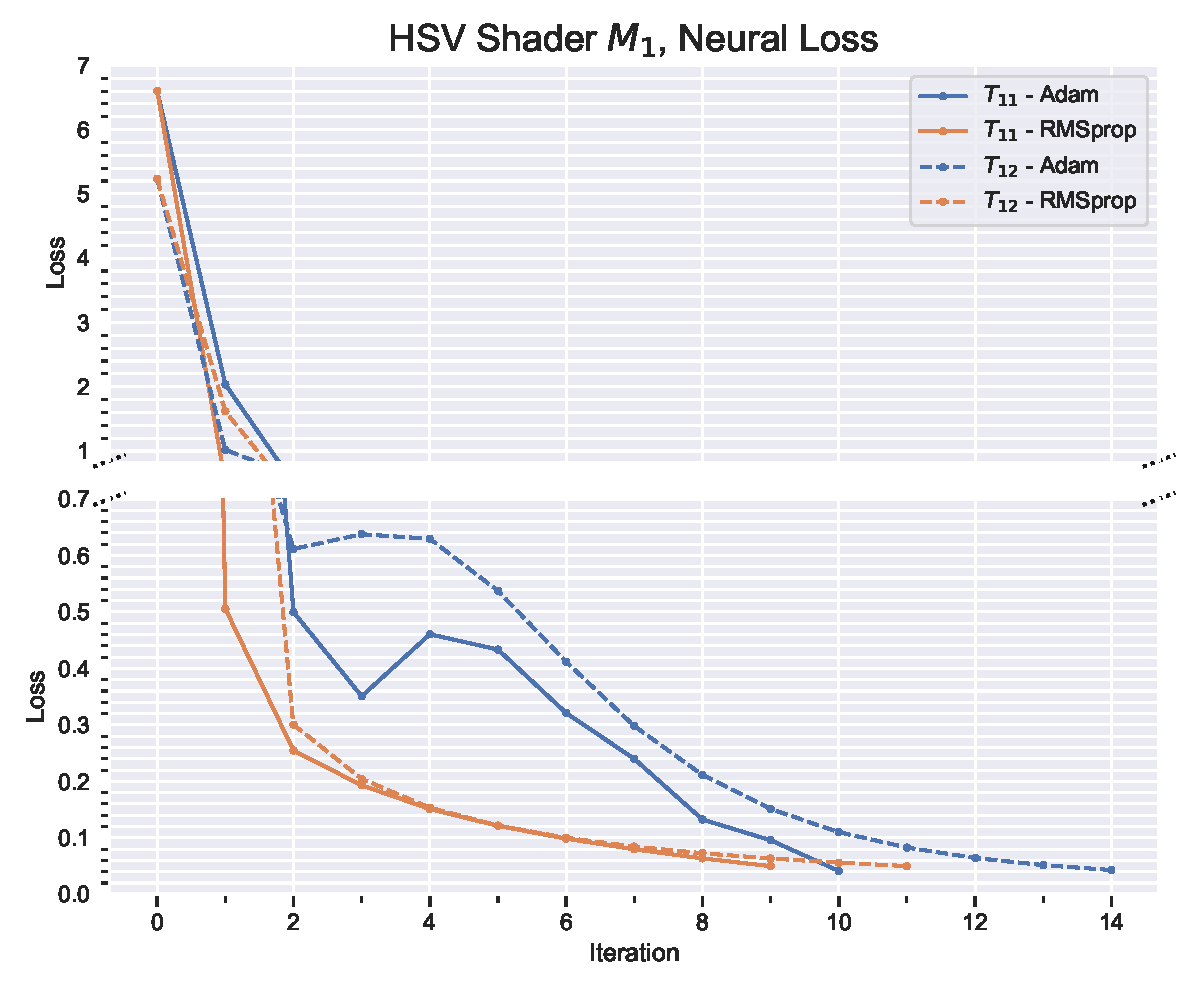
\includegraphics[width=0.8\textwidth]{img/evaluation/M1/HSV_NEURAL.pdf}
    \caption{Results of evaluating parameter estimation of material $M_1$ using Neural loss. The runs with target $T_{11}$ are plotted as solid lines and target $T_{12}$ with dashed lines.}
    \label{fig:M1NeuralData}
\end{figure}

\begin{figure}[hpb]
\centering
\begin{subfigure}[t]{.25\textwidth}
    \centering
    
\includegraphics[width=\linewidth]{img/evaluation/M1/2 param/Neural_Adam_final_render.png}
    \caption{Target $T_{11}$ using Adam.}
    \label{fig:M1NeuralFinalRenders2paramAdam}
\end{subfigure}\hspace{0.7cm}
\begin{subfigure}[t]{.25\textwidth}
    \centering
    
\includegraphics[width=\linewidth]{img/evaluation/M1/random/Neural_Adam_random_final.png}
    \caption{Target $T_{12}$ using Adam.}
    \label{fig:M1NeuralFinalRendersRandomAdam}
\end{subfigure}
\vskip\baselineskip
\begin{subfigure}[t]{.25\textwidth}
    \centering
    
\includegraphics[width=\linewidth]{img/evaluation/M1/2 param/Neural_RMSprop_final_render.png}
    \caption{Target $T_{11}$ using RMSprop.}
    \label{fig:M1NeuralFinalRenders2paramRMSprop}
\end{subfigure}\hspace{0.7cm}
\begin{subfigure}[t]{.25\textwidth}
    \centering
    
\includegraphics[width=\linewidth]{img/evaluation/M1/random/Neural_RMSprop_random_final.png}
    \caption{Target $T_{12}$ using RMSprop.}
    \label{fig:M1NeuralFinalRendersRandomRMSprop}
\end{subfigure}
\caption{The four rendered textures at the point of minimal loss for $M_1$ using Neural loss corresponding to the four plots in Figure \ref{fig:M1NeuralData} with combinations of optimizers Adam or RMSprop and targets $T_{11}$ or $T_{12}$.}
\label{fig:M1NeuralFinalRenders}
\end{figure}

\subsubsection{Simple Brick Shader $M_2$}

The results of running gradient descent on test shader $M_2$ using a neural loss function are shown in Figure \ref{fig:M2NeuralData} where the initial loss when running parameter estimation using Adam with target $T_{21}$ is relatively high. As shown in table \ref{tab:NeuralLossOptimizerSettings}, we used a different set of layers to extract features from when running with target $T_{21}$ using Adam, which is reflected in Figure \ref{fig:M2NeuralData}, as it yielded much better results. It is interesting that the single layer 0 works well for RMSprop, but gave very poor results with Adam. This is probably due to RMSprop by chance finding a better path to a minimum and we could have probably reached the same results with Adam had we explored a much wider range of optimizer settings. Using Adam and target $T_{21}$ we were able to reach a minimum loss of $0.07$ at iteration 341 and with RMSprop a minimum loss of $0.004$ at iteration 334. The renders at these points of minimal loss are shown in subfigures \ref{fig:M2NeuralFinalRenders2paramAdam} and \ref{fig:M2NeuralFinalRenders2paramRMSprop} respectively where a slightly better result was achieved by using RMSprop but is surprisingly not much better than using a simple MSE loss. The color was retrieved fairly well but the elongation is only about 60\% of the target. The real advantage of using a neural loss is instead reflected in the cases with the random target $T_{22}$ where the initial loss starts at around $0.3$ and is minimized down to $0.02$ for Adam at iteration 381 and $0.036$ for RMSprop at iteration 21. While RMSprop is clearly much faster to reach convergence, the results are better for Adam as seen in subfigures \ref{fig:M2NeuralFinalRendersRandomRMSprop} and \ref{fig:M2NeuralFinalRendersRandomAdam} respectively. As opposed to using a MSE loss or SBL the shape of the bricks were actually retained and even elongated when using Adam, although not nearly as much as in the target. Clearly a neural loss is a better choice for pattern heavy images, especially when optimizing a large number of parameters, although it is still difficult to reproduce the exact shape.

\begin{figure}[h]
    \centering
    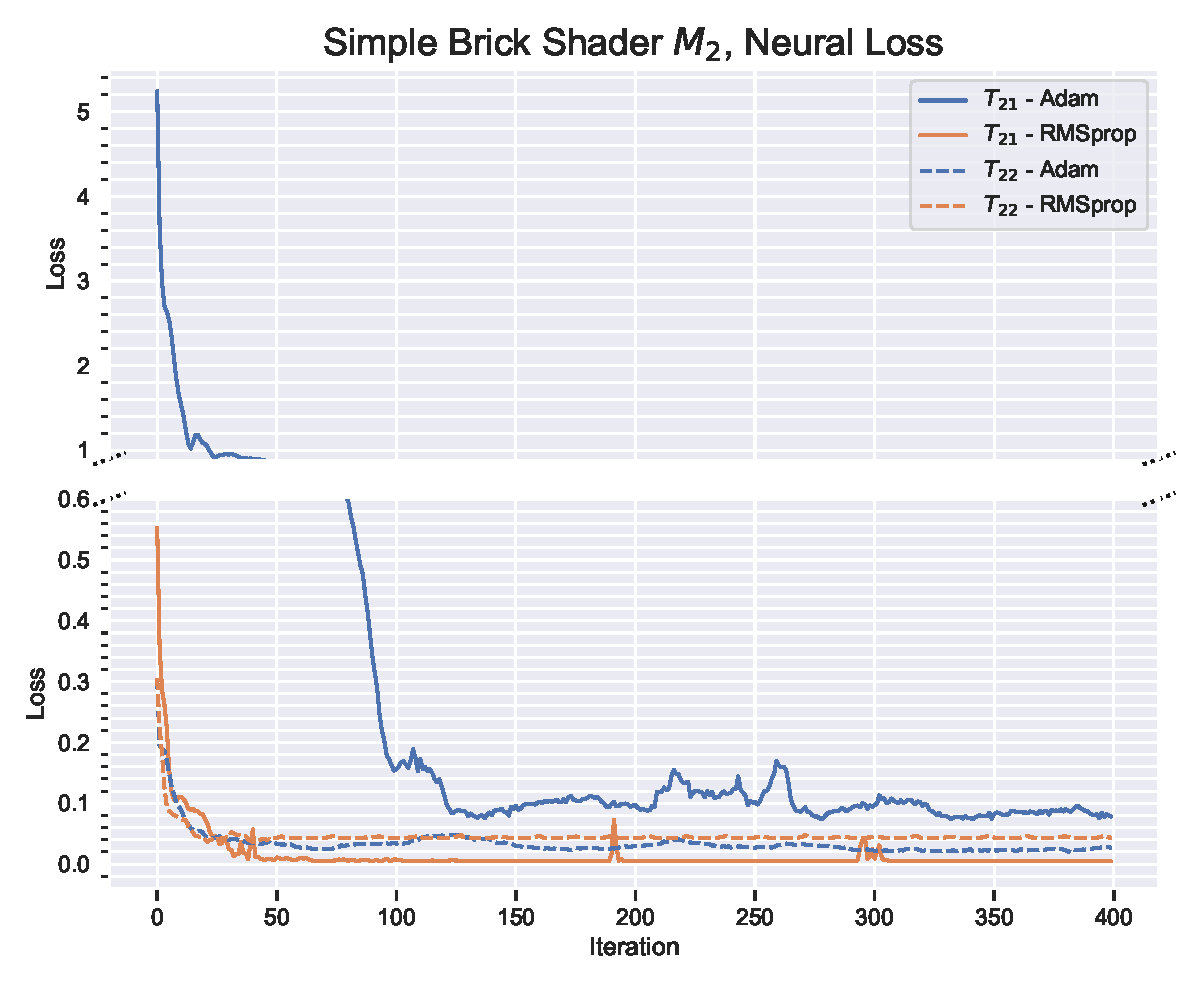
\includegraphics[width=0.8\textwidth]{img/evaluation/M2/SBS_Neural.pdf}
    \caption{Results of evaluating parameter estimation of material $M_2$ using Neural loss. The runs with target $T_{21}$ are plotted as solid lines while runs with target $T_{22}$ are plotted with dashed lines.}
    \label{fig:M2NeuralData}
\end{figure}

\begin{figure}[h]
\centering
\begin{subfigure}[t]{.25\textwidth}
    \centering
    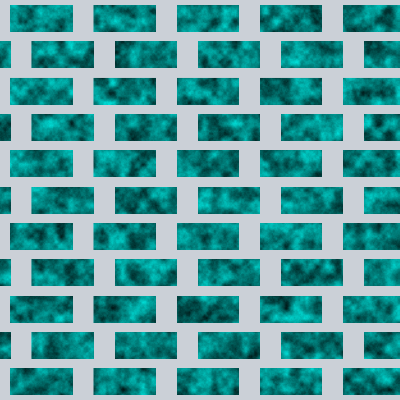
\includegraphics[width=\linewidth]{img/evaluation/M2/2param/Neural_Adam_final_render.png}
    \caption{Target $T_{21}$ using Adam.}
    \label{fig:M2NeuralFinalRenders2paramAdam}
\end{subfigure}\hspace{0.5cm}
\begin{subfigure}[t]{.25\textwidth}
    \centering
    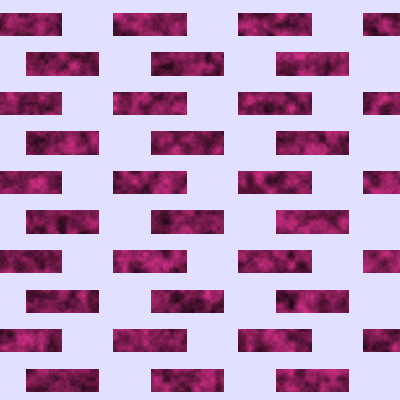
\includegraphics[width=\linewidth]{img/evaluation/M2/random/Neural_Adam_Random_best.png}
    \caption{Target $T_{22}$ using Adam.}
    \label{fig:M2NeuralFinalRendersRandomAdam}
\end{subfigure}
\vskip\baselineskip
\begin{subfigure}[t]{.25\textwidth}
    \centering
    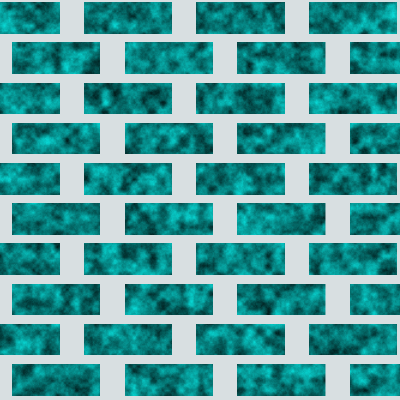
\includegraphics[width=\linewidth]{img/evaluation/M2/2param/Neural_RMSprop_final_render.png}
    \caption{Target $T_{21}$ using RMSprop.}
    \label{fig:M2NeuralFinalRenders2paramRMSprop}
\end{subfigure}
\hspace{0.5cm}
\begin{subfigure}[t]{.25\textwidth}
    \centering
    \includegraphics[width=\linewidth]{img/evaluation/M2/random/Neural_RMSprop_Random_best.png}
    \caption{Target $T_{22}$ using RMSprop.}
    \label{fig:M2NeuralFinalRendersRandomRMSprop}
\end{subfigure}
\caption{The four rendered textures at the point of minimal loss for $M_2$ using Neural corresponding to the six plots in Figure \ref{fig:M2NeuralData} with combinations of optimizers Adam or RMSprop and targets $T_{21}$ or $T_{32}$.}
\label{fig:M2NeuralFinalRenders}
\end{figure}


\subsubsection{Advanced Brick Test Shader $M_3$}

\begin{figure}[h]
    \centering
    \includegraphics[width=0.8\textwidth]{img/evaluation/M3/ABS_NEURAL.pdf}
    \caption{Results of evaluating parameter estimation of material $M_3$ using Neural loss. The runs with target $T_{31}$ are plotted as solid lines, target $T_{32}$ with dashed lines and the additional real-life target $T_{33}$ with dotted lines.}
    \label{fig:M3NeuralData}
\end{figure}

\begin{figure}[h]
\centering
\begin{subfigure}[t]{.25\textwidth}
    \centering
    \includegraphics[width=\linewidth]{img/evaluation/M3/2 param/Neural_Adam_2_param.png}
    \caption{Target $T_{31}$ using Adam.}
    \label{fig:M3NeuralFinalRendersTwoParamAdam}
\end{subfigure}\hspace{0.7cm}
\begin{subfigure}[t]{.25\textwidth}
    \centering
    \includegraphics[width=\linewidth]{img/evaluation/M3/random/Neural_Adam_random_final.png}
    \caption{Target $T_{32}$ using Adam.}
    \label{fig:M3NeuralFinalRendersRandomAdam}
\end{subfigure}\hspace{0.7cm}
\begin{subfigure}[t]{.25\textwidth}
    \centering
    \includegraphics[width=\linewidth]{img/evaluation/M3/real life/Neural_Adam_real_life_final.png}
    \caption{Target $T_{33}$ using Adam.}
    \label{fig:M3NeuralFinalRendersRealLifeAdam}
\end{subfigure}
\vskip\baselineskip
\begin{subfigure}[t]{.25\textwidth}
    \centering
    \includegraphics[width=\linewidth]{img/evaluation/M3/2 param/Neural_RMSprop_2_param.png}
    \caption{Target $T_{31}$ using RMSprop.}
    \label{fig:M3NeuralFinalRendersTwoParamRMSprop}
\end{subfigure}\hspace{0.7cm}
\begin{subfigure}[t]{.25\textwidth}
    \centering
    \includegraphics[width=\linewidth]{img/evaluation/M3/random/Neural_RMSprop_random_final.png}
    \caption{Target $T_{32}$ using RMSprop.}
    \label{fig:M3NeuralFinalRendersRandomRMSprop}
\end{subfigure}\hspace{0.7cm}
\begin{subfigure}[t]{.25\textwidth}
    \centering
    \includegraphics[width=\linewidth]{img/evaluation/M3/real life/Neural_RMSprop_real_life_final.png}
    \caption{Target $T_{33}$ using RMSprop.}
    \label{fig:M3NeuralFinalRendersRealLifeRMSprop}
\end{subfigure}
\caption{The six rendered textures at the point of minimal loss for $M_3$ using Neural loss corresponding to the six plots in Figure \ref{fig:M3NeuralData} with combinations of optimizers Adam or RMSprop and targets $T_{31}$, $T_{32}$ or $T_{33}$.}
\label{fig:M3NeuralFinalRenders}
\end{figure}

Finally, we evaluate parameter estimation on $M_3$ using a neural loss function where the loss data is shown in Figure \ref{fig:M3NeuralData}. As seen in table \ref{tab:NeuralLossOptimizerSettings}, this case necessitated the use of a range of different settings for the neural loss function. Interestingly enough, there were big differences in performances between the two optimizers depending on which layers were used. Most notably for target $T_{31}$, where the same learning rate was used for both optimizers, but we only used layer $4$ for RMSprop and only layer $5$ for Adam as the reverse resulted in both optimizers performing much worse. The loss per iteration for $T_{31}$ is plotted using solid lines, and we can recognize a familiar pattern: RMSprop converges much earlier than Adam with a minimum loss of $0.0014$ at iteration 164 while Adam reaches a minimum loss of $0.009$ at iteration 397. Note that we can not directly compare the final loss values as we use different layers but the final renders shown in subfigures \ref{fig:M3NeuralFinalRendersTwoParamAdam} and \ref{fig:M3NeuralFinalRendersTwoParamRMSprop} respectively makes it clear that the result for Adam is superior. Both optimizers successfully retain the overall color of the target, but only Adam manages to correctly retain the scale, albeit at the expense of correct brick elongation. 

The loss data for the random target $T_{32}$ is plotted using dashed lines where both optimizers experience a fairly unstable few initial iterations. However, in this case RMSprop not only converges much earlier at iteration 192 versus Adam that does not converge at all, the minimum loss for RMSprop is much lower at $0.05$ against $0.13$ for Adam where both used layer $0$ with the same weights for the neural loss. Judging the resulting renders in subfigures \ref{fig:M3NeuralFinalRendersRandomAdam} for Adam and \ref{fig:M3NeuralFinalRendersRandomRMSprop} for RMSprop however, its difficult to see much similarity between either and the target.

The last and perhaps most interesting target $T_{33}$ is represented as dotted line plots where the additional layer $4$ was used for Adam which did not seem to provide any benefits for RMSprop. Both manage to quite successfully minimize the loss where Adam reached a minimum value of $0.2$ at iteration 363 and RMS a minimum value of $0.19$ at iteration 340. Furthermore, Adam experienced a much smoother progression whereas RMSprop saw several large spikes which might be preventable with better tuned learning rate and $\alpha$ parameters. The rendered results are shown in subfigures \ref{fig:M3NeuralFinalRendersRealLifeAdam} and \ref{fig:M3NeuralFinalRendersRealLifeRMSprop}, proving that the overall color has been very well reproduced in both cases, even the color of the mortar. What differentiates both cases is the scale of the bricks, where Adam managed to achieve better similarity, but again, both results show too elongated bricks. Furthermore, the noise function influencing the color of the bricks has not been changed much, although that could be the fault of the shader model composition itself. Ultimately, using a real life texture worked well but required a fair amount of tuning of optimizer and loss parameters.

Overall, the results are much better than when using MSE loss or SBL and except for target $T_{32}$, the overall color was very well retained, and when using Adam even the scale of the bricks was fairly well restored, although the elongation of the bricks remains a difficult problem to solve for both optimizers. For this case, Adam is the superior optimizer, although only marginally.


\subsection{Finding a ''Correct'' Minimum}

We have demonstrated that using gradient descent and a differentiable rendering system we can easily minimize a loss function applied to a static bitmap target and a generated image. However, there are no guarantees that the minimum found is a global minimum, or even that a low loss value corresponds to a high image similarity. In the end, the similarity is judged by a human user with a subjective idea of what constitutes similar images. Using a neural loss function is a big step in the right direction but in order to make judgements for other kinds of shaders, further evaluation is needed.

We impose practical limits on parameter values when controlled by the user, which can introduce problems during parameter estimation. For example, the hue, value and saturation parameters of the HSV shader are all limited to the interval $[0,1]$. The reason being that the hue parameter is cyclical meaning a value of 1.5 is equivalent to 0.5 while the saturation and value parameters are effectively capped to the interval so that a negative value is equivalent to 0 and any value > 1 is equivalent to 1. PyTorch tensors do not support such limits and neither do the optimizers. It would be possible to develop a custom optimizer that clamps parameters to their intervals, but this will inevitably have a negative impact on the optimization as a whole. Figure \ref{fig:HSVShaderLossSurface} shows the loss surface generated by evaluating the MSE loss of shader $M_1$ over a range of hue and saturation values using target $T_{11}$, as well as the gradient descent progress. A magenta plus symbol marks the minimum loss value and markers along the gradient descent route indicates each iteration. This proves the cyclic behaviour of the hue value as the loss is repeated along the x-axis. This means that we have one minimum every \texttt{hue=0.3,1.3,2.3} etc and because the initial value of the hue is 1.0, the closest minimum for the optimizer to seek is the one where \texttt{hue=1.3}, which unfortunately is outside of our limits, and simply clamping this value would result in a worse loss with \texttt{hue=1.0}.

\begin{figure}[h]
    \centering
    \includegraphics[width=0.8\textwidth]{img/evaluation/HSV Shader Loss Surface.pdf}
    \caption{Loss surface generated by evaluating an MSE loss between shader $M_1$ and target $T_{11}$ for a range of different \texttt{hue} and \texttt{value} parameter values. A magenta ''plus'' symbol denotes the point of minimum loss and the red line marks the gradient descent progress.}
    \label{fig:HSVShaderLossSurface}
\end{figure}
